\documentclass[10pt]{article}

% Double-blind TMLR submission mode (change to [preprint] or [accepted] for camera-ready)
\usepackage{tmlr}

\usepackage{amsmath,amssymb}
\usepackage{booktabs}
\usepackage{makecell}
\usepackage[section]{placeins}
\usepackage{graphicx}
\usepackage{hyperref}
\usepackage{pifont}
\usepackage{xcolor}
\usepackage{microtype}
\usepackage{listings}

\hypersetup{
  colorlinks=true,
  linkcolor=blue!50!black,
  citecolor=blue!50!black,
  urlcolor=blue!50!black
}

\lstset{
  basicstyle=\ttfamily\footnotesize,
  breaklines=true,
  frame=single,
  columns=fullflexible,
  keepspaces=true
}

% Double-blind toggle
\newif\ifblind
\blindtrue

% Include Appendices A--F in the same PDF (standard for TMLR)
\newif\ifincludeappendix
\includeappendixtrue

\newcommand{\cmark}{\ding{51}}
\newcommand{\xmark}{\ding{55}}
\newcommand{\repoRef}{%
  \ifblind
    the anonymized supplementary archive%
  \else
    the project repository%
  \fi
}

% Auto-generated Study 3, E5, and E6 statistics (zero hand-typed numbers)
% Auto-generated by openreview/build_macros.py. Do not edit by hand.
% Sources: derived/study3/study3.json, E5 summary.json, E6 summary.json.

\newcommand{\sThreeTotalGames}{16,000}
\newcommand{\sThreeGamesPerModel}{3,200}
\newcommand{\sThreePoneGemma}{$+$0.114}
\newcommand{\sThreePoneCIGemma}{[$+$0.100, $+$0.129]}
\newcommand{\sThreePonePGemma}{$< 0.001$}
\newcommand{\sThreeAzeroGemma}{$-$0.238}
\newcommand{\sThreeAzeroAbsGemma}{0.238}
\newcommand{\sThreeAzeroCIGemma}{[$-$0.261, $-$0.215]}
\newcommand{\sThreeAzeroPGemma}{$< 0.001$}
\newcommand{\sThreeAoneGemma}{$+$0.002}
\newcommand{\sThreeAoneCIGemma}{[$-$0.010, $+$0.014]}
\newcommand{\sThreeAonePGemma}{$0.950$}
\newcommand{\sThreeKappaGemma}{$-$0.027}
\newcommand{\sThreeKappaCIGemma}{[$-$0.034, $-$0.021]}
\newcommand{\sThreeOmegaGemma}{$-$0.240}
\newcommand{\sThreeDeltaMGemma}{$-$0.253}
\newcommand{\sThreePthreeBGemma}{$+$0.013}
\newcommand{\sThreeSoneAzeroGemma}{$-$0.156}
\newcommand{\sThreeStwoAGemma}{$-$0.129}
\newcommand{\sThreeStwoBGemma}{$-$0.109}
\newcommand{\sThreeStwoBPGemma}{$< 0.001$}
\newcommand{\sThreeSfiveRhoGemma}{0.85}
\newcommand{\sThreeSsixHighGemma}{$-$0.039}
\newcommand{\sThreeSsixHighPGemma}{$0.055$}
\newcommand{\sThreeSnineAoneLowGemma}{0.98}
\newcommand{\sThreeSnineAoneHighGemma}{0.97}
\newcommand{\sThreeSnineShiftRhoGemma}{$+$0.51}
\newcommand{\sThreeForfeitsGemma}{0}
\newcommand{\sThreeTimeoutsGemma}{0}
\newcommand{\sThreeTrailingGemma}{0}
\newcommand{\sThreeOutsideGemma}{0}
\newcommand{\sThreePoneQwen}{$+$0.101}
\newcommand{\sThreePoneCIQwen}{[$+$0.089, $+$0.113]}
\newcommand{\sThreePonePQwen}{$< 0.001$}
\newcommand{\sThreeAzeroQwen}{$+$0.029}
\newcommand{\sThreeAzeroAbsQwen}{0.029}
\newcommand{\sThreeAzeroCIQwen}{[$+$0.001, $+$0.058]}
\newcommand{\sThreeAzeroPQwen}{$0.115$}
\newcommand{\sThreeAoneQwen}{$+$0.077}
\newcommand{\sThreeAoneCIQwen}{[$+$0.059, $+$0.094]}
\newcommand{\sThreeAonePQwen}{$< 0.001$}
\newcommand{\sThreeKappaQwen}{$-$0.001}
\newcommand{\sThreeKappaCIQwen}{[$-$0.007, $+$0.006]}
\newcommand{\sThreeOmegaQwen}{$-$0.016}
\newcommand{\sThreeDeltaMQwen}{$+$0.007}
\newcommand{\sThreePthreeBQwen}{$-$0.023}
\newcommand{\sThreeSoneAzeroQwen}{$-$0.117}
\newcommand{\sThreeStwoAQwen}{$+$0.037}
\newcommand{\sThreeStwoBQwen}{$-$0.007}
\newcommand{\sThreeStwoBPQwen}{$1.000$}
\newcommand{\sThreeSfiveRhoQwen}{0.83}
\newcommand{\sThreeSsixHighQwen}{$-$0.069}
\newcommand{\sThreeSsixHighPQwen}{$< 0.001$}
\newcommand{\sThreeSnineAoneLowQwen}{0.93}
\newcommand{\sThreeSnineAoneHighQwen}{0.93}
\newcommand{\sThreeSnineShiftRhoQwen}{$+$0.03}
\newcommand{\sThreeForfeitsQwen}{0}
\newcommand{\sThreeTimeoutsQwen}{0}
\newcommand{\sThreeTrailingQwen}{0}
\newcommand{\sThreeOutsideQwen}{20}
\newcommand{\sThreePoneLuna}{$+$0.048}
\newcommand{\sThreePoneCILuna}{[$+$0.034, $+$0.062]}
\newcommand{\sThreePonePLuna}{$< 0.001$}
\newcommand{\sThreeAzeroLuna}{$-$0.129}
\newcommand{\sThreeAzeroAbsLuna}{0.129}
\newcommand{\sThreeAzeroCILuna}{[$-$0.147, $-$0.112]}
\newcommand{\sThreeAzeroPLuna}{$< 0.001$}
\newcommand{\sThreeAoneLuna}{$-$0.030}
\newcommand{\sThreeAoneCILuna}{[$-$0.044, $-$0.016]}
\newcommand{\sThreeAonePLuna}{$0.002$}
\newcommand{\sThreeKappaLuna}{$-$0.032}
\newcommand{\sThreeKappaCILuna}{[$-$0.039, $-$0.026]}
\newcommand{\sThreeOmegaLuna}{$-$0.093}
\newcommand{\sThreeDeltaMLuna}{$-$0.105}
\newcommand{\sThreePthreeBLuna}{$+$0.011}
\newcommand{\sThreeSoneAzeroLuna}{$-$0.101}
\newcommand{\sThreeStwoALuna}{$-$0.079}
\newcommand{\sThreeStwoBLuna}{$-$0.050}
\newcommand{\sThreeStwoBPLuna}{$< 0.001$}
\newcommand{\sThreeSfiveRhoLuna}{0.84}
\newcommand{\sThreeSsixHighLuna}{$-$0.002}
\newcommand{\sThreeSsixHighPLuna}{$0.796$}
\newcommand{\sThreeSnineAoneLowLuna}{0.89}
\newcommand{\sThreeSnineAoneHighLuna}{0.93}
\newcommand{\sThreeSnineShiftRhoLuna}{$+$0.56}
\newcommand{\sThreeForfeitsLuna}{35}
\newcommand{\sThreeTimeoutsLuna}{23}
\newcommand{\sThreeTrailingLuna}{616}
\newcommand{\sThreeOutsideLuna}{0}
\newcommand{\sThreePoneHaiku}{$-$0.020}
\newcommand{\sThreePoneCIHaiku}{[$-$0.041, $+$0.003]}
\newcommand{\sThreePonePHaiku}{$0.985$}
\newcommand{\sThreeAzeroHaiku}{$-$0.051}
\newcommand{\sThreeAzeroAbsHaiku}{0.051}
\newcommand{\sThreeAzeroCIHaiku}{[$-$0.077, $-$0.026]}
\newcommand{\sThreeAzeroPHaiku}{$0.014$}
\newcommand{\sThreeAoneHaiku}{$-$0.113}
\newcommand{\sThreeAoneCIHaiku}{[$-$0.131, $-$0.096]}
\newcommand{\sThreeAonePHaiku}{$< 0.001$}
\newcommand{\sThreeKappaHaiku}{$-$0.044}
\newcommand{\sThreeKappaCIHaiku}{[$-$0.054, $-$0.034]}
\newcommand{\sThreeOmegaHaiku}{$+$0.016}
\newcommand{\sThreeDeltaMHaiku}{$-$0.023}
\newcommand{\sThreePthreeBHaiku}{$+$0.038}
\newcommand{\sThreeSoneAzeroHaiku}{$-$0.105}
\newcommand{\sThreeStwoAHaiku}{$-$0.019}
\newcommand{\sThreeStwoBHaiku}{$-$0.033}
\newcommand{\sThreeStwoBPHaiku}{$0.110$}
\newcommand{\sThreeSfiveRhoHaiku}{0.37}
\newcommand{\sThreeSsixHighHaiku}{$+$0.002}
\newcommand{\sThreeSsixHighPHaiku}{$0.883$}
\newcommand{\sThreeSnineAoneLowHaiku}{0.83}
\newcommand{\sThreeSnineAoneHighHaiku}{0.82}
\newcommand{\sThreeSnineShiftRhoHaiku}{$+$0.07}
\newcommand{\sThreeForfeitsHaiku}{0}
\newcommand{\sThreeTimeoutsHaiku}{0}
\newcommand{\sThreeTrailingHaiku}{0}
\newcommand{\sThreeOutsideHaiku}{77}
\newcommand{\sThreePoneGemini}{$+$0.195}
\newcommand{\sThreePoneCIGemini}{[$+$0.175, $+$0.214]}
\newcommand{\sThreePonePGemini}{$< 0.001$}
\newcommand{\sThreeAzeroGemini}{$-$0.295}
\newcommand{\sThreeAzeroAbsGemini}{0.295}
\newcommand{\sThreeAzeroCIGemini}{[$-$0.346, $-$0.245]}
\newcommand{\sThreeAzeroPGemini}{$< 0.001$}
\newcommand{\sThreeAoneGemini}{$+$0.100}
\newcommand{\sThreeAoneCIGemini}{[$+$0.083, $+$0.119]}
\newcommand{\sThreeAonePGemini}{$< 0.001$}
\newcommand{\sThreeKappaGemini}{$+$0.005}
\newcommand{\sThreeKappaCIGemini}{[$-$0.002, $+$0.012]}
\newcommand{\sThreeOmegaGemini}{$-$0.340}
\newcommand{\sThreeDeltaMGemini}{$-$0.308}
\newcommand{\sThreePthreeBGemini}{$-$0.032}
\newcommand{\sThreeSoneAzeroGemini}{$-$0.247}
\newcommand{\sThreeStwoAGemini}{$-$0.213}
\newcommand{\sThreeStwoBGemini}{$-$0.082}
\newcommand{\sThreeStwoBPGemini}{$< 0.001$}
\newcommand{\sThreeSfiveRhoGemini}{0.83}
\newcommand{\sThreeSsixHighGemini}{$-$0.097}
\newcommand{\sThreeSsixHighPGemini}{$< 0.001$}
\newcommand{\sThreeSnineAoneLowGemini}{0.75}
\newcommand{\sThreeSnineAoneHighGemini}{0.93}
\newcommand{\sThreeSnineShiftRhoGemini}{$+$0.40}
\newcommand{\sThreeForfeitsGemini}{0}
\newcommand{\sThreeTimeoutsGemini}{0}
\newcommand{\sThreeTrailingGemini}{0}
\newcommand{\sThreeOutsideGemini}{120}
\newcommand{\sThreeSnineMin}{0.75}
\newcommand{\sThreeSnineMax}{0.98}
\newcommand{\sThreeSnineShiftMin}{$+$0.40}
\newcommand{\sThreeSnineShiftMax}{$+$0.56}
\newcommand{\sThreePredictionsMet}{21}
\newcommand{\sThreePredictionsTotal}{25}
\newcommand{\eFiveGapShare}{17\%}
\newcommand{\eFiveSwapFortyOne}{75\%}
\newcommand{\eFiveSwapFortyTwo}{83\%}
\newcommand{\eFiveReplyShare}{57\%}
\newcommand{\eFivePromptShare}{22\%}
\newcommand{\eFiveBuyerProbMass}{0.32}
\newcommand{\eFiveHeadOverlap}{6}
\newcommand{\eFiveHeldOutMoved}{$-$12.56}
\newcommand{\eFiveHeldOutRatio}{1.88}
\newcommand{\eFiveHeldOutOwnGapPct}{67\%}
\newcommand{\eFiveHeldOutRandMoved}{$-$0.06}
\newcommand{\eFiveSteerAoneLow}{32\%}
\newcommand{\eFiveSteerAoneHigh}{44\%}
\newcommand{\eFiveSteerAzeroLow}{89\%}
\newcommand{\eFiveSteerAzeroHigh}{92\%}
\newcommand{\eSixNegMove}{86\%}
\newcommand{\eSixNegRand}{8\%}
\newcommand{\eSixRiskNatGap}{10.0}
\newcommand{\eSixRiskMove}{5\%}
\newcommand{\eSixRiskCtrl}{2\%}
\newcommand{\eSixPctMove}{$-$4\%}
\newcommand{\eSixPctCtrl}{$-$2\%}
\newcommand{\eSixFermiPlus}{1.15}
\newcommand{\eSixFermiMinus}{0.50}
\newcommand{\eSixCos}{0.32}
\newcommand{\addDOneGames}{640}
\newcommand{\addDOneMeanThought}{274.9}
\newcommand{\addDOneOutside}{0}
\newcommand{\addDOneAzeroD}{$-$0.178}
\newcommand{\addDOneAzeroDCI}{[$-$0.210, $-$0.146]}
\newcommand{\addDOneAzeroDP}{$< 0.001$}
\newcommand{\addDOneAzeroDelta}{$+$0.116}
\newcommand{\addDOneAzeroDeltaP}{$0.008$}
\newcommand{\addDOneAzeroH}{$-$0.204}
\newcommand{\addDOneAoneD}{$+$0.065}
\newcommand{\addDOneAoneDCI}{[$+$0.046, $+$0.083]}
\newcommand{\addDOneAoneDP}{$< 0.001$}
\newcommand{\addDOneAoneDelta}{$-$0.036}
\newcommand{\addDOneAoneDeltaP}{$0.003$}
\newcommand{\addDOnePoneI}{$+$0.145}
\newcommand{\addDOnePoneICI}{[$+$0.131, $+$0.159]}
\newcommand{\addDThreeGames}{320}
\newcommand{\addDThreeD}{$-$0.167}
\newcommand{\addDThreeDCI}{[$-$0.236, $-$0.101]}
\newcommand{\addDThreeDP}{$< 0.001$}
\newcommand{\addDThreeDelta}{$+$0.127}
\newcommand{\addDThreeDeltaCI}{[$+$0.066, $+$0.188]}
\newcommand{\addDOneGemmaGames}{80}
\newcommand{\addDOneGemmaNFx}{20}
\newcommand{\addDOneGemmaD}{$-$0.332}
\newcommand{\addDOneGemmaDCI}{[$-$0.410, $-$0.256]}
\newcommand{\addDOneGemmaDP}{$< 0.001$}
\newcommand{\addDOneGemmaH}{$-$0.131}
\newcommand{\addDOneQwenGames}{80}
\newcommand{\addDOneQwenH}{$-$0.184}
\newcommand{\addDOneQwenHP}{$0.008$}
\newcommand{\eSixBRiskMass}{1.00}
\newcommand{\eSixBRiskShare}{$-$4\%}
\newcommand{\eSixBRiskShareOne}{0\%}
\newcommand{\eSixBPctShare}{$+$3\%}
\newcommand{\eSixBNegShare}{$+$18\%}


\title{Multiply by a Million: Scale Invariance in LLM Negotiators}

% Author block is automatically replaced by "Anonymous authors" under \usepackage{tmlr}
\author{\name Anonymous Authors \\
\addr Under double-blind review}

\newcommand{\fix}{\marginpar{FIX}}
\newcommand{\new}{\marginpar{NEW}}

\begin{document}

\maketitle

\begin{abstract}
People take more risk with small stakes and discount large amounts less; we ask whether LLM negotiators, whose task is identical at every scale, also respond to scale. We test this in a locally frozen, hash-verified confirmatory study of five models (Gemma 4 31B, Qwen3.8 27B, \texttt{gpt-6-luna}, \texttt{claude-haiku-5.5}, and \texttt{gemini-3.5-flash-lite}), each playing \sThreeGamesPerModel{} self-play games (\sThreeTotalGames{} total) on 40 randomly drawn price ranges at \$100, \$100K, and \$100M, with and without a public appraisal of the lot and with an opening clamp that scripts both first offers. Without the appraisal, every model opens closer to its own limit at \$100M. On all five models, deals follow the scripted openings' midpoint within $\pm 0.05$ of the surplus. The appraisal reduces the opening effect on four models and removes Gemma's closing shift (from \sThreeAzeroGemma{} to \sThreeAoneGemma{} of the surplus), but it is not a general remedy: it reverses the shift on Gemini (\sThreeAoneGemini{}) and enlarges it on Haiku (\sThreeAoneHaiku{}). Exploratory controls across 10{,}000+ additional games on Gemma 4 31B and Qwen3.8 27B show that explicit scale-neutral instructions fail to eliminate opening shrinkage, both digit-string length and unit words contribute independently (even when cents are shown), and asymmetric cross-model play exposes high-shrinkage sellers to surplus loss. A preregistered post-Study 3 robustness check (Addendum D, 960 games on Gemini across the same 40 fixtures) further shows that enabling native thinking (\addDOneMeanThought{} thinking tokens/call) attenuates but does not eliminate either opening modesty (\addDOneAzeroH{}) or the A0 closing shift (\addDOneAzeroD{}, $p$ \addDOneAzeroDP{}), preserves the A1 sign reversal (\addDOneAoneD{}), and that replacing \$100 with \$1{,}000 still leaves a large negative shift (\addDThreeD{}, $p$ \addDThreeDP{}). Mechanistically, an exploratory analysis finds that the appraisal takes over Gemma's opening at layer 41 of 60, on the tokens that write the price, through attention heads that largely overlap the scale and private-range circuits, while the scale direction behaves more like numerical magnitude than a cross-task risk preference. Ultimately, evaluating an agent at one numerical scale does not certify it at another.
\end{abstract}

\section{Introduction}

People do not treat a bargain a million times larger as the same bargain. They gamble on small stakes and turn cautious on large ones \citep{markowitz1952utility, weber2005peanuts}, grow more risk averse as payoffs are scaled up \citep{holt2002risk}, and discount large delayed amounts less than small ones \citep{thaler1981empirical}; \citet{prelec1991decision} trace these effects to a common source. Large language models learn from human text and may inherit such stake effects.

LLM agents are increasingly evaluated as negotiators \citep{bianchi2024negotiationarena, abdelnabi2024scoreable, zhu2026piearena}, usually within one range of prices. A basic robustness question is whether the same bargain, written with every monetary amount a million times larger, produces the same relative offers and the same division of surplus. For negotiators whose utility is linear in money, rescaling leaves the Nash and Rubinstein solutions unchanged \citep{nash1950bargaining, rubinstein1982perfect}; a person with concave utility need not be indifferent. Our task removes that reason. It gives the negotiator no wealth, budget, or time cost, only a private limit and the goal of the best price, so a deal at the same share of the surplus is equally good at every scale. Invariance is the benchmark the task itself sets, and a departure means the model brings in a stake effect, or a number-handling effect, that the task does not ask for.

One observed bargain shows what can go wrong (Figure~\ref{fig:main-game}). Gemma 4 31B, selling with a private floor of \$83 to a buyer with a ceiling of \$118, opened at \$120 and kept 69\% of the surplus. With limits of \$83M and \$118M, the same words, and the same sampling seed, it opened at \$95M and kept 11\%.

\begin{figure}[t]
  \centering
  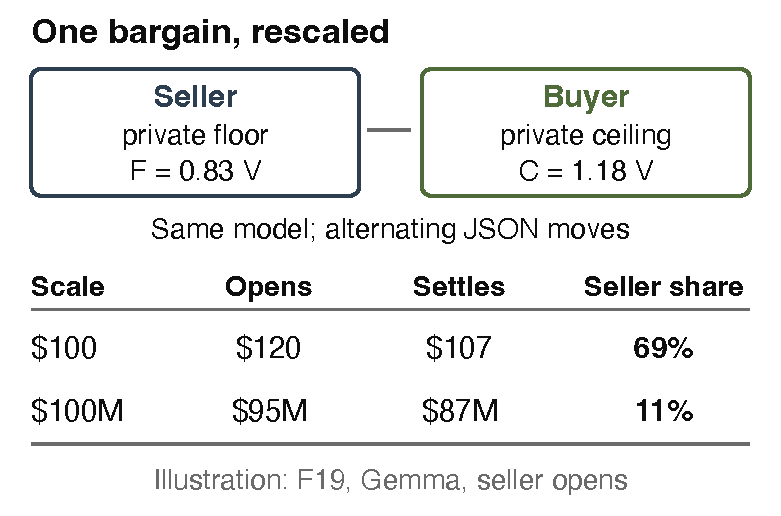
\includegraphics[width=0.72\textwidth]{../manuscript/figures/main_game.pdf}
  \caption{A fixed-geometry bargaining test. The same fixture rescaled from \$100 to \$100M. Each side sees only its own limit; both openers are tested. The game shown is from the discovery phase (Gemma, Study 2, fixture F19, seller opening) and illustrates the question; the evidence comes from paired comparisons across fixtures.}
  \label{fig:main-game}
\end{figure}

Earlier exploratory and registered studies of this game (the discovery phase, Section~\ref{sec:hypotheses} and Appendix~\ref{app:discovery}) suggested a specific account: at large amounts the opener asks for less; deals settle near the midpoint of the two first offers; and a public reference number such as an appraisal may remove the effect. This paper reports Study 3, a single account, under one protocol, on five models and on bargains no earlier run used. Its hypotheses, analysis code, and scripted opening values were frozen and hashed before the first game, and every registered test is reported.

We find:
\begin{itemize}
  \item \textbf{Opening modesty at scale is shared (Section~\ref{sec:res-openings}).} Without the appraisal, all five models open closer to their own limit at \$100M than at \$100. The appraisal reduces this on four models; on Haiku it does not.
  \item \textbf{Closing shifts follow the openings (Section~\ref{sec:res-clamp}).} Scripting both first offers at their \$100M positions shifts deals by the change in the scripted midpoint, within $\pm 0.05$ of the surplus, on all five models (informatively on Gemma, Luna, and Gemini); with the openings fixed, concessions add a small shift on Gemma and Luna and a larger one on Haiku.
  \item \textbf{A reference number is not a general fix (Section~\ref{sec:res-closing}).} The appraisal removes Gemma's shift and shrinks Luna's, but reverses Gemini's and enlarges Haiku's.
  \item \textbf{Prompting, notation, and cross-play controls constrain simple workarounds (Section~\ref{sec:res-controls}, exploratory).} Across 10{,}000+ exploratory games, explicit scale-neutral instructions fail to eliminate opening shrinkage; both digit strings and unit words contribute even when cents are displayed; and asymmetric cross-play confirms surplus loss when a high-shrinkage seller faces a more scale-stable buyer.
  \item \textbf{Inside Gemma, the reference takes over late (Section~\ref{sec:interp}, exploratory).} The appraisal becomes decisive at layer 41 of 60, on the reply's price-writing tokens, through attention heads that largely also carry the scale and private-range effects, while the scale signal persists with less effect on the price.
  \item \textbf{The scale signal looks like numerical magnitude, not stakes (Section~\ref{sec:e6}, exploratory).} Gemma reads amounts on one number line in five notations and loses its preference for better gambles at \$100M, but the direction that shifts its openings moves its risky choices by only \eSixRiskMove{} of that gap.
\end{itemize}

The scope is specific: five models, one prompt family, one single-issue game, and self-play with thinking off or minimised in the main confirmatory Study 3 (supplemented by exploratory cross-play in Section~\ref{sec:res-controls} and preregistered thinking-on, 3-model cross-play, and \$1{,}000 anchor checks in Section~\ref{sec:res-addendum-d}). We separate registered primary tests, registered secondaries, and exploratory analyses throughout.

\section{Related work}

Inside bargaining theory, the more risk-averse party receives less under the Nash solution \citep{kihlstrom1981risk}, so a stake-dependent risk attitude is one route by which scale could move a split. Human bargaining studies find mixed stake-size effects \citep{andersen2011stakes, larney2019stakesize, karagozoglu2017stakesize}. For LLMs, multiplying every payoff in a repeated Prisoner's Dilemma while preserving its structure produces model-specific responses \citep{huynh2026payoff}; dictator and ultimatum studies likewise find heterogeneous stake effects \citep{polachek2026stakes, araujo2026ultimatum}. We extend the fixed-structure manipulation to a continuous price negotiated over multiple turns.

LLM negotiators have been studied in self-play and in arenas \citep{fu2023selfplay, bianchi2024negotiationarena, abdelnabi2024scoreable, zhu2026piearena}. Two bargaining studies vary the value at stake, and in both the magnitude moves together with the geometry: doubling a retail price with cost fixed triples the margin \citep{liang2026supplychain}, and limits drawn from items' historical prices make the dollar level and the width of the zone of agreement vary together \citep{bergemann2026bilateral}. A self-play study that varies the zone's width finds model-specific crossovers between buyer and seller advantage \citep{rios2025illusion}; a house-sale study varies whether a description of the house and comparable sales are shown, close to our appraisal contrast, but not the magnitude \citep{shah2025rationalis}.

First offers predict negotiated outcomes in people \citep{galinsky2001first, schweinsberg2023firstoffer, lipp2023anchorzone} and can anchor LLM negotiations \citep{takenami2025anchoring}. This motivates the midpoint account but does not establish it for our game, which the opening clamp tests directly. Inside models, number values are linearly decodable \citep{zhu2024valuelinear}, alongside digit-wise and helical codes \citep{levy2024digit, kantamneni2025trigonometry}; irrelevant numeric anchors have been localised to sparse circuits whose depth differs by model family \citep{owusu2026anchoring}. Our mechanistic methods build on activation patching and difference-vector steering \citep{heimersheim2024patching, turner2023actadd, zou2023repe}.

\section{Hypotheses and where they came from}
\label{sec:hypotheses}

Study 3's hypotheses were generated in a discovery phase of two registered studies, three registered addenda, and exploratory probes, all reported in Appendix~\ref{app:discovery}. Table~\ref{tab:discovery-map} lists what each suggested and which Study 3 test checks it. No discovery data enter a primary test; they fix only the hypotheses, the margins, and the scripted opening values, and the descriptive secondary S8 compares Study 3 with them.

\begin{table}[t]
  \centering
  \caption{From discovery to confirmation. Discovery-phase observations fix Study 3's hypotheses, equivalence margins, and scripted opening values; no discovery data enter any Study 3 primary test.}
  \label{tab:discovery-map}
  \small
  \begin{tabular}{@{}p{0.42\textwidth}p{0.31\textwidth}p{0.21\textwidth}@{}}
    \toprule
    Discovery-phase observation & Source (Appendix~\ref{app:discovery}) & Study 3 test \\
    \midrule
    Without an appraisal, openers move toward their own limit at \$100M & Qwen Study 2 (exploratory); Addendum A on Gemma and Addendum B on three API models (registered) & S1 ($h(\text{A0}) < 0$) \\
    With the appraisal and both limit ranges shown, Qwen's openings and split did not move & Qwen Study 1; probe X10 & P1 (appraisal alone attenuates opening modesty) \\
    Without an appraisal, closing splits shift on Gemma, Luna, and Gemini, and meet $\pm 0.10$ equivalence on Qwen and Haiku & Study 2; Addendum C & P2, A0 \\
    Deals close near the midpoint of the two first offers; prospectively supported on Luna only & Study 2 (exploratory); Addendum C (registered) & P3b; S5 \\
    Telling both sides the other's range nearly pinned Gemma's openings but left a concession residual & Probes X26--X27 & P3a ($\kappa$) \\
    The scale effect in Gemma becomes decisive near layer 41, on the reply's price tokens & Interpretability X52--X62 & E5 (exploratory, predictions committed) \\
    \bottomrule
  \end{tabular}
\end{table}

Two gaps in the discovery phase motivated a new study rather than another addendum. In the registered studies, Gemma and the API models never saw an appraisal, so the remedy had been tested only on Qwen, together with the limit ranges. And the protocol changed between runs (one game per cell or four, blocked or interleaved order, 512 or 1{,}024 output tokens), so cross-model comparisons were confounded with procedure.

\section{Study 3 design}
\label{sec:design}

\paragraph{Game.} Two copies of a model negotiate one price. The seller knows a private floor $F$, the buyer a private ceiling $C$, and both know a deal is possible ($F < C$). They alternate JSON moves (\texttt{OFFER} a whole-dollar price, \texttt{ACCEPT} the standing offer, or \texttt{WALKAWAY}) with a message of at most 500 characters, for at most 16 messages. Each call is rebuilt from the rules, the side's own limit, and the public history. Invalid replies forfeit the game without repair. For a deal at $P$, seller share is $s = (P - F)/(C - F)$.

\paragraph{Fixtures and scales.} Forty fresh fixtures (G01--G40) from a public seeded generator place floors at 75--95\% and ceilings at 105--125\% of a reference value $V$. Each is played at $V = \$100$, $\$100\text{K}$, and $\$100\text{M}$. Money is always written as digits followed by ``dollars''; with the digits masked, the prompts at the three scales are identical.

\paragraph{Conditions (Table~\ref{tab:s3-design}).} The core grid crosses the appraisal (A0: no appraisal, Study 2's prompt; A1: one added line, ``An independent appraisal values the lot at $V$. Both sides know this.'') with scale and opener. The opening clamp, in A0 only, scripts both first offers into the public history and lets the model begin playing at message 3, at game scale $G$ across the scripted opening scale $O$. The scripted positions are each model's mean first-offer positions in its own earlier no-appraisal games, in zone units. At \$100M they are the \$100 prices with six zeros appended.

\begin{table}[t]
  \centering
  \caption{Study 3 cells per model ($k = 4$ games per cell, both openers, 40 fixtures).}
  \label{tab:s3-design}
  \small
  \begin{tabular}{@{}llr@{}}
    \toprule
    Block & Cells & Games per model \\
    \midrule
    Core grid & appraisal (A0, A1) $\times$ scale (\$100, \$100K, \$100M) & 1,920 \\
    Opening clamp (A0) & game scale $G$ (\$100, \$100M) $\times$ scripted opening scale $O$ (\$100, \$100M) & 1,280 \\
    \midrule
    Total & 10 cells $\times$ 2 openers $\times$ 40 fixtures $\times$ 4 & \sThreeGamesPerModel{} \\
    \bottomrule
  \end{tabular}
\end{table}

\paragraph{Models.} Qwen3.8 27B (FP8) and Gemma 4 31B (bf16) run on pinned weights in vLLM 0.30.0 with each family's non-thinking sampling settings and no repetition penalties. \texttt{gpt-6-luna}, \texttt{claude-haiku-5.5}, and \texttt{gemini-3.5-flash-lite} (hereafter Luna, Haiku, and Gemini) run through OpenRouter on each vendor's own endpoint with vendor sampling defaults and thinking off; Gemini's lowest setting, ``minimal'', does not guarantee zero reasoning, so its reasoning tokens were counted (none were reported). Sampling stays model-native; ``one protocol'' means every procedural rule is identical. Seeds are shared across scale, appraisal, and clamp cell, so every within-fixture contrast shares them (Anthropic receives none; Appendix~\ref{app:protocol}).

\paragraph{Sessions.} Each model ran in two independent sessions (samples 1--2 and 3--4): separate GPU pods for the open-weight models, separate days for the API models. Each session interleaved all cells in one fixed shuffle.

\paragraph{Tests.} The fixture is the unit of analysis; a cell's value is the mean over its four games (agreements only, for seller share).
\begin{itemize}
  \item \textbf{P1 (openings).} With $g$ the opener's first-offer gap from its own limit, $h_f(A) = \text{mean over openers of } g(\$100\text{M}) - g(\$100)$, and $I_f = h_f(\text{A1}) - h_f(\text{A0})$. One-sided Wilcoxon, $I > 0$.
  \item \textbf{P2 (closing shift).} $d_i = s(\$100\text{M}) - s(\$100)$, averaged over openers, per condition. A two-sided Wilcoxon (H1) and equivalence if the 90\% bootstrap CI lies within $\pm 0.10$ (H2) \citep{lakens2017tostprimer}. A non-significant H1 is never read as equivalence.
  \item \textbf{P3 (decomposition, A0).} The concession channel $\kappa$ is the scale effect with both openings held at the same scripted positions, averaged over the opening scale; ``openings suffice'' predicts $\kappa$ equivalent to zero within $\pm 0.05$. The opening channel $\omega$ is the effect of moving the scripted openings from their \$100 to their \$100M positions, averaged over the game scale; ``deals follow the scripted midpoint'' predicts $\omega - \Delta m$ equivalent to zero within $\pm 0.05$, where $\Delta m$ is the shift in the scripted offers' midpoint.
\end{itemize}

Wilcoxon $p$-values use 200{,}000 random sign flips; bootstrap intervals resample fixtures 10{,}000 times; Holm correction runs across the five models within each test. Nine registered secondaries (S1--S9) are reported in Appendix~\ref{app:study3-full}.

\paragraph{Registration and data access.} The registration, the files the study executes or reads (37 in all, including the analysis code and the scripted opening values), and their SHA-256 hashes were committed before any registered game; every session recorded the commit and checked the hashes. The registration was not lodged with an external registry (Appendix~\ref{app:reg}). Format pilots on separate fixtures were judged on format only. One rule was set after the first API pilot, which was then rerun under it, and before the freeze: text after the first complete JSON object is ignored and flagged, rather than forfeiting the game. After the open-weight sessions, and before the second API session, we looked at Gemma and Qwen through the frozen analysis; this access was committed to a log first, the API outcome data stayed unexamined, and nothing in the protocol changed (Appendix~\ref{app:reg}).

\section{Results}
\label{sec:results}

All \sThreeTotalGames{} games were scored and every game record reproduces exactly from the raw calls. Luna forfeited \sThreeForfeitsLuna{} games (34 truncated replies); no other model forfeited. Outside-zone agreements (retained unclipped as registered) occurred on Gemini (\sThreeOutsideGemini{}), Haiku (\sThreeOutsideHaiku{}), and Qwen (\sThreeOutsideQwen{}), with zero on Gemma and Luna (cell-level breakdown in Appendix~\ref{app:study3-full}; all-game seller utility S3 confirms the primary shifts). Table~\ref{tab:s3-primary} scores every registered primary test against its prediction: \sThreePredictionsMet{} of \sThreePredictionsTotal{} are met.

% Auto-generated from derived/study3/study3.json
\begin{table}[t]
\centering
\caption{Registered primary tests, Study 3. Mean over 40 fixtures [90\% bootstrap CI]; $p$: Wilcoxon signed-rank (200{,}000 sign flips), Holm across the five models (P1 one-sided). Predictions (registration \S5.1): P1 $I > 0$ on all five; P2 A0 a shift on Gemma, Luna, and Gemini (two-sided) and equivalence within $\pm 0.10$ on Qwen and Haiku; P2 A1 equivalence within $\pm 0.10$ on all five; P3a $\kappa$ and P3b $\omega - \Delta m$ equivalent to zero within $\pm 0.05$ (90\% CI). A non-significant test is never read as equivalence. Total: 21 of 25.}
\label{tab:s3-primary}
\scriptsize
\setlength{\tabcolsep}{4pt}
\resizebox{\textwidth}{!}{%
\begin{tabular}{@{}lccccc@{}}
\toprule
Model & P1 $\cdot$ $I > 0$ & P2 $\cdot$ A0 shift/equiv. & P2 $\cdot$ A1 equiv. & P3a $\cdot$ $\kappa \approx 0$ & P3b $\cdot$ $\omega - \Delta m \approx 0$ \\
\midrule
Gemma 4 31B & \makecell{\cmark $+$0.114 ($p$ $< 0.001$) \\{} [$+$0.100, $+$0.129]} & \makecell{\cmark $-$0.238 ($p$ $< 0.001$) (n.e.) \\{} [$-$0.261, $-$0.215]} & \makecell{\cmark $+$0.002 ($p$ $0.950$) \\{} [$-$0.010, $+$0.014]} & \makecell{\cmark $-$0.027 ($p$ $< 0.001$) \\{} [$-$0.034, $-$0.021]} & \makecell{\cmark $+$0.013 \\{} [$+$0.001, $+$0.024]} \\
\addlinespace[2pt]
Qwen3.8 27B & \makecell{\cmark $+$0.101 ($p$ $< 0.001$) \\{} [$+$0.089, $+$0.113]} & \makecell{\cmark $+$0.029 ($p$ $0.115$) \\{} [$+$0.001, $+$0.058]} & \makecell{\cmark $+$0.077 ($p$ $< 0.001$) \\{} [$+$0.059, $+$0.094]} & \makecell{\cmark $-$0.001 ($p$ $0.799$) \\{} [$-$0.007, $+$0.006]} & \makecell{\cmark $-$0.023 \\{} [$-$0.030, $-$0.016]} \\
\addlinespace[2pt]
gpt-6-luna & \makecell{\cmark $+$0.048 ($p$ $< 0.001$) \\{} [$+$0.034, $+$0.062]} & \makecell{\cmark $-$0.129 ($p$ $< 0.001$) (n.e.) \\{} [$-$0.147, $-$0.112]} & \makecell{\cmark $-$0.030 ($p$ $0.002$) \\{} [$-$0.044, $-$0.016]} & \makecell{\cmark $-$0.032 ($p$ $< 0.001$) \\{} [$-$0.039, $-$0.026]} & \makecell{\cmark $+$0.011 \\{} [$+$0.004, $+$0.018]} \\
\addlinespace[2pt]
claude-haiku-5.5 & \makecell{\xmark $-$0.020 ($p$ $0.985$) \\{} [$-$0.041, $+$0.003]} & \makecell{\cmark $-$0.051 ($p$ $0.014$) \\{} [$-$0.077, $-$0.026]} & \makecell{\xmark $-$0.113 ($p$ $< 0.001$) \\{} [$-$0.131, $-$0.096]} & \makecell{\xmark $-$0.044 ($p$ $< 0.001$) \\{} [$-$0.054, $-$0.034]} & \makecell{\cmark $+$0.038 \\{} [$+$0.029, $+$0.047]} \\
\addlinespace[2pt]
gemini-3.5-flash-lite & \makecell{\cmark $+$0.195 ($p$ $< 0.001$) \\{} [$+$0.175, $+$0.214]} & \makecell{\cmark $-$0.295 ($p$ $< 0.001$) (n.e.) \\{} [$-$0.346, $-$0.245]} & \makecell{\xmark $+$0.100 ($p$ $< 0.001$) \\{} [$+$0.083, $+$0.119]} & \makecell{\cmark $+$0.005 ($p$ $0.340$) \\{} [$-$0.002, $+$0.012]} & \makecell{\cmark $-$0.032 \\{} [$-$0.044, $-$0.019]} \\
\addlinespace[2pt]
\midrule
\textbf{Predictions met} & \textbf{4 of 5} & \textbf{5 of 5} & \textbf{3 of 5} & \textbf{4 of 5} & \textbf{5 of 5} \\
\bottomrule
\end{tabular}%
}
\end{table}


\subsection{Openings shrink at scale; the appraisal attenuates this on four models}
\label{sec:res-openings}

Without the appraisal, every model's opener moves toward its own limit at \$100M (S1: $h$ from \sThreeSoneAzeroLuna{} on Luna to \sThreeSoneAzeroGemini{} on Gemini, all Holm-adjusted $p < 0.001$; Figure~\ref{fig:s3-openings}). The registered appraisal $\times$ scale interaction $I$ is positive on Gemma (\sThreePoneGemma{}), Qwen (\sThreePoneQwen{}), Luna (\sThreePoneLuna{}), and Gemini (\sThreePoneGemini{}). On Haiku it is \sThreePoneHaiku{} (90\% CI \sThreePoneCIHaiku{}): with the appraisal shown, Haiku's sellers open at 0.55 of their floor above it at \$100 and 0.31 at \$100M, a steeper fall than without it. Only on Qwen does the remaining opening change meet the $\pm 0.03$ equivalence margin.

\begin{figure}[t]
  \centering
  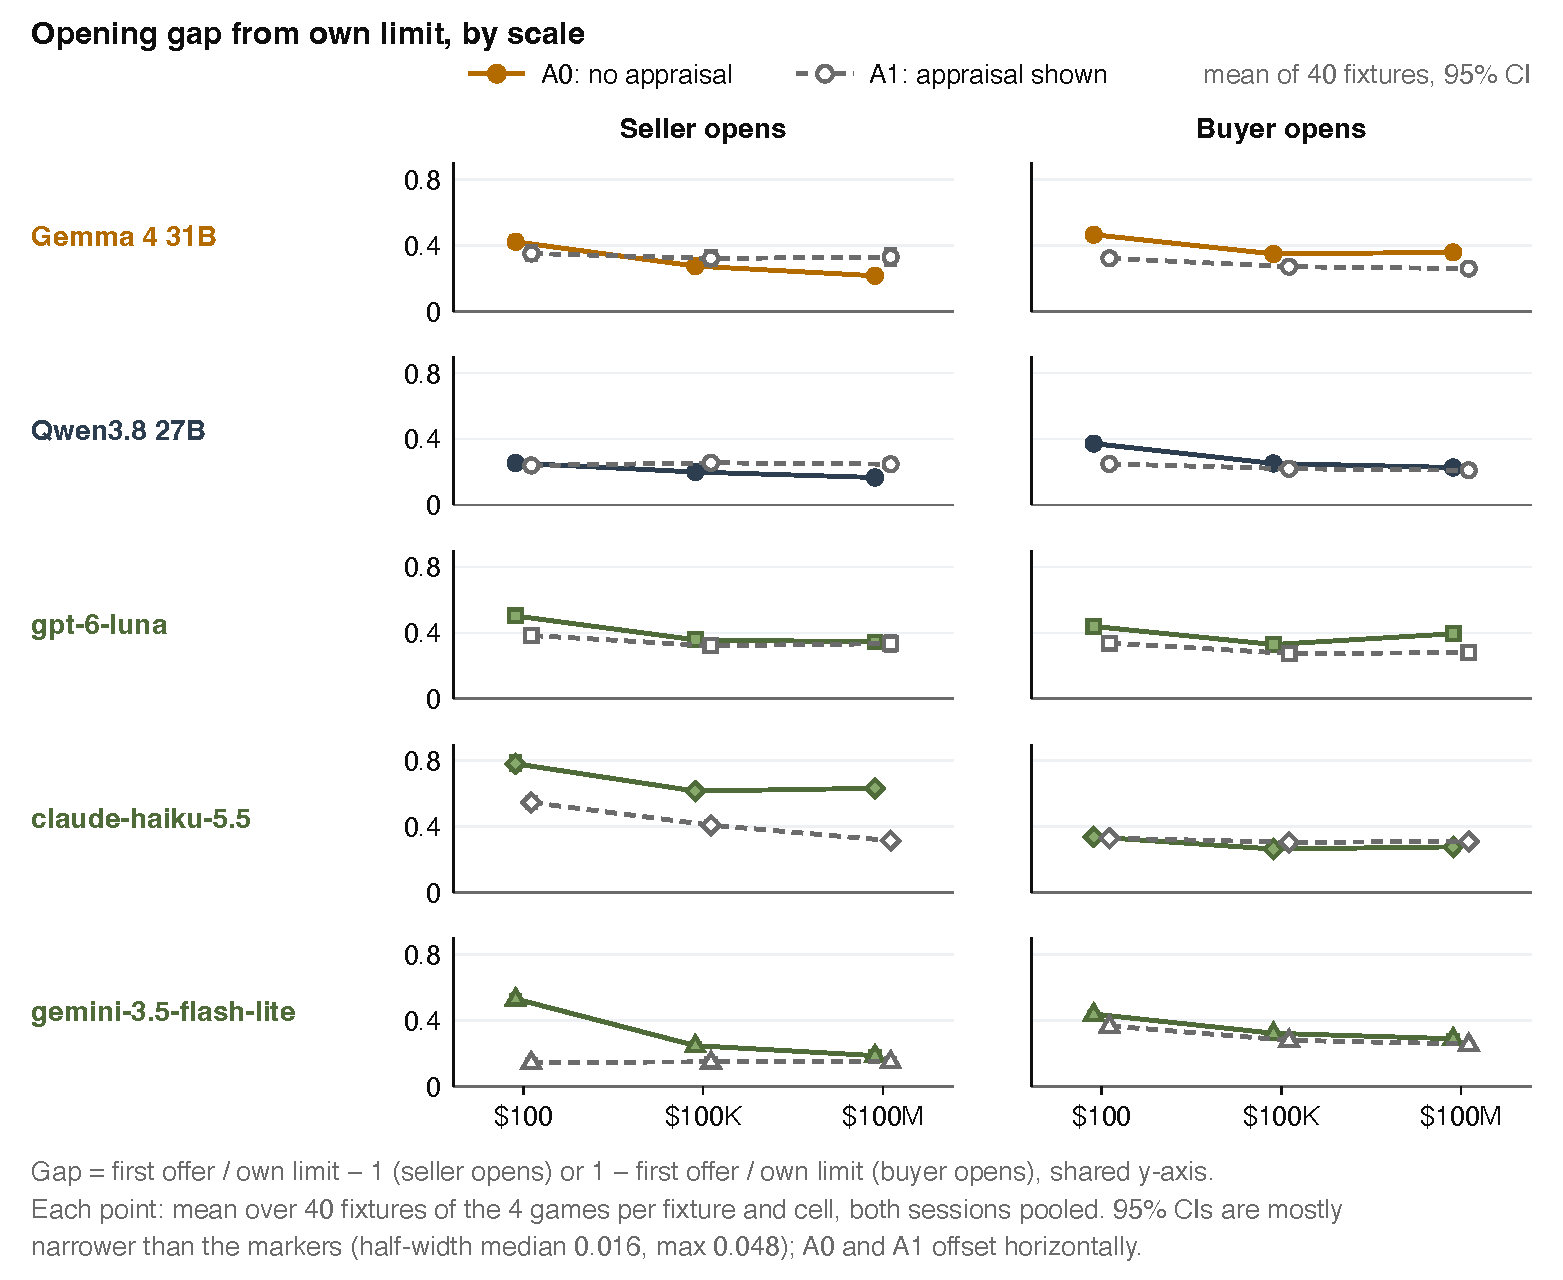
\includegraphics[width=0.95\textwidth]{../manuscript/figures/s3_openings.pdf}
  \caption{Opening modesty by scale, with and without the appraisal. The opener's first-offer gap from its own limit at each scale (seller: $\text{ask} / F - 1$; buyer: $1 - \text{offer} / C$), mean over 40 fixtures with 95\% CIs. Solid: no appraisal (A0); dashed: appraisal shown (A1). P1 compares the $\$100\text{M} - \$100$ change between conditions; the \$100K point is descriptive.}
  \label{fig:s3-openings}
\end{figure}

With the appraisal shown, Gemma's and Qwen's sellers open at a level that hardly moves with scale. Gemini's sellers open close to the appraisal itself (a gap of about 0.15 at every scale), while its buyers still drift toward their ceiling at large amounts.

\subsection{Closing shifts: as predicted without the appraisal, model-dependent with it}
\label{sec:res-closing}

Without the appraisal, the closing shift matches the registered prediction on all five models (Figure~\ref{fig:s3-shift}): seller share falls by \sThreeAzeroAbsGemma{} on Gemma, \sThreeAzeroAbsLuna{} on Luna, and \sThreeAzeroAbsGemini{} on Gemini, while Qwen (\sThreeAzeroQwen{}) and Haiku (\sThreeAzeroHaiku{}) meet equivalence within $\pm 0.10$. Haiku's shift is also significantly below zero (Holm $p =$ \sThreeAzeroPHaiku{}) and larger than in the discovery phase (S8: $+0.006$ in Addendum C). Registered adjacent-scale contrasts (S2, Table~\ref{tab:s3-sec-a}) confirm that the no-appraisal shift is not solely an artefact of \$100 whole-dollar discretization: moving from \$100K to \$100M (where \$1 is $10^{-5}$ of $V$) still significantly lowers seller share on Gemma (\sThreeStwoBGemma{}), Luna (\sThreeStwoBLuna{}), and Gemini (\sThreeStwoBGemini{}, all within-model Holm $p < 0.001$).

\begin{figure}[t]
  \centering
  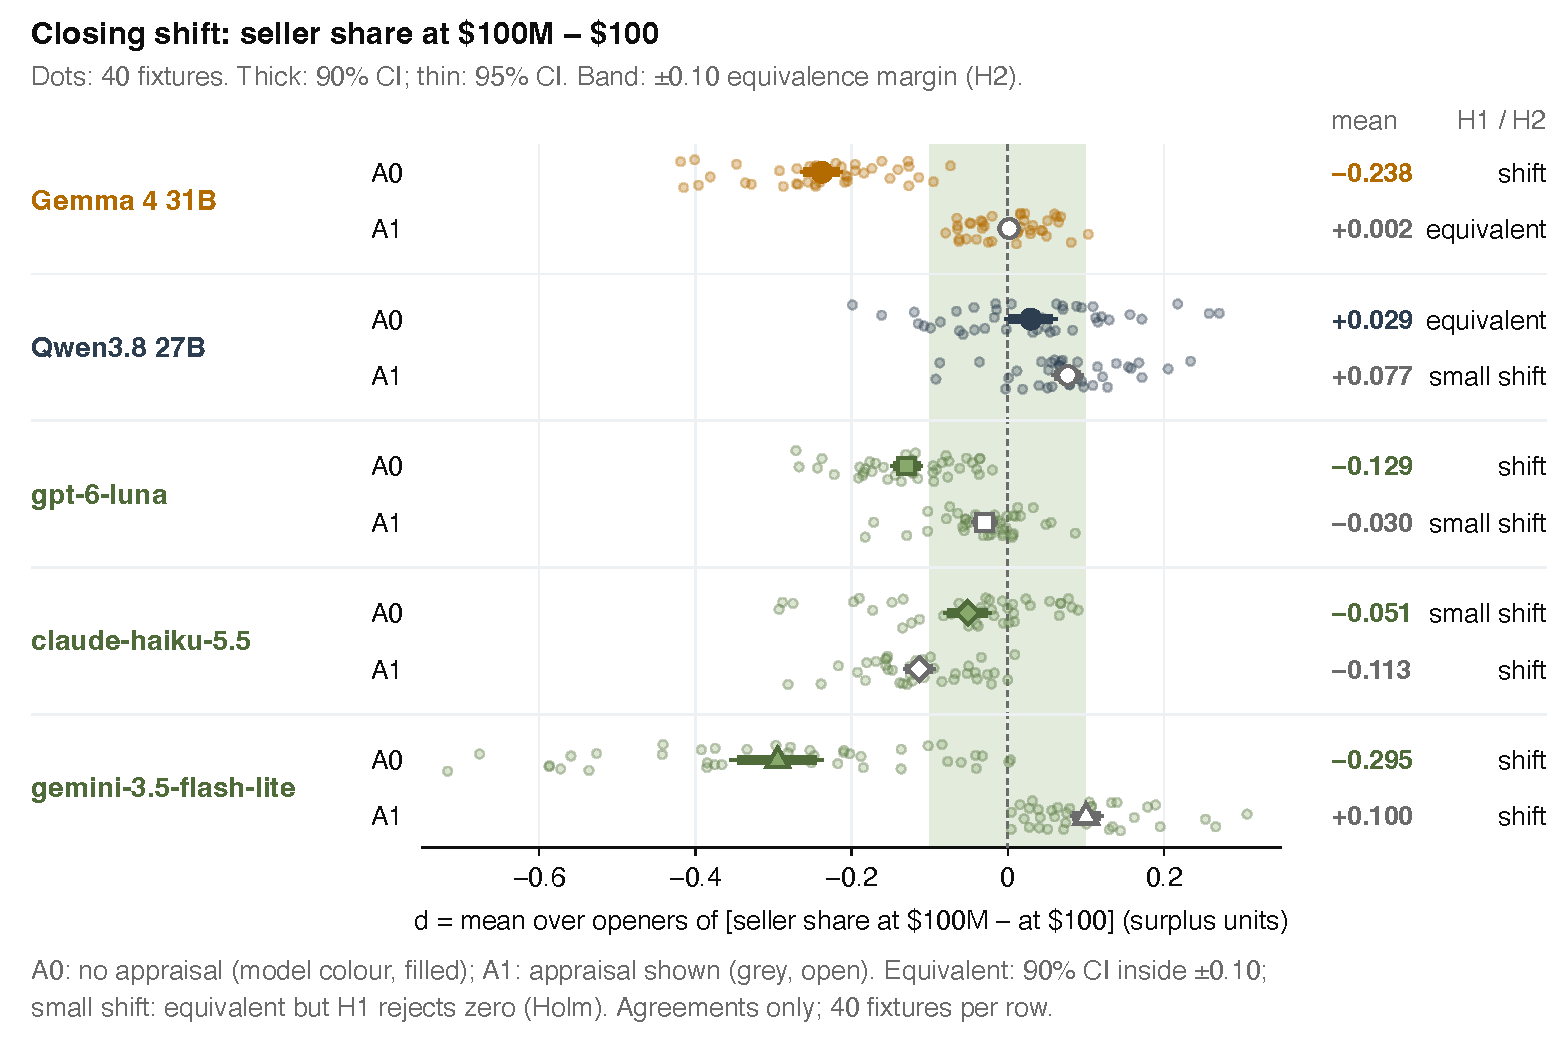
\includegraphics[width=0.95\textwidth]{../manuscript/figures/s3_shift.pdf}
  \caption{Closing shift by model and appraisal condition (P2). Seller share at \$100M minus at \$100, per fixture (dots), with the mean, 90\% CI (thick), and 95\% CI (thin). Band: the registered $\pm 0.10$ equivalence margin.}
  \label{fig:s3-shift}
\end{figure}

With the appraisal, the prediction of equivalence on all five fails on two. Gemma's shift vanishes (\sThreeAoneGemma{} \sThreeAoneCIGemma{}). Qwen (\sThreeAoneQwen{}) and Luna (\sThreeAoneLuna{}) meet equivalence but show small, significant shifts. Gemini's shift reverses (\sThreeAoneGemini{} \sThreeAoneCIGemini{}): its sellers open next to the appraisal at every scale and settle low at \$100, while its buyers open closer to their ceiling at \$100M, so deals settle higher there. Haiku's shift grows (\sThreeAoneHaiku{} \sThreeAoneCIHaiku{}), consistent with its sellers' collapsing openings. In every model, deals under the appraisal track where the appraisal sits in the zone (S9: Spearman \sThreeSnineMin{}--\sThreeSnineMax{} across fixtures), so the appraisal works as an anchor; whether that anchor removes the scale effect depends on how each model's openings respond to it. On Gemma, Luna, and Gemini the shift under the appraisal also rises with the appraisal's position in the zone (S9, $\rho$ \sThreeSnineShiftMin{} to \sThreeSnineShiftMax{}; descriptive).

\subsection{The opening clamp: deals follow the openings}
\label{sec:res-clamp}

The clamp separates two channels (Figure~\ref{fig:s3-clamp}). Moving the scripted openings from their \$100 to their \$100M positions, with the game's scale averaged out, shifts the deal by the amount the scripted midpoint predicts on every model, informatively on Gemma, Luna, and Gemini (P3b: $\omega - \Delta m$ within $\pm 0.05$ on all five). On Gemma, for example, $\omega =$ \sThreeOmegaGemma{} against $\Delta m =$ \sThreeDeltaMGemma{}, close to its natural shift of \sThreeAzeroGemma{}; on Gemini, \sThreeOmegaGemini{} against \sThreeDeltaMGemini{} and a natural \sThreeAzeroGemini{}. On Qwen and Haiku both terms are near zero, so P3b cannot distinguish its predictions there, as anticipated in the registration.

\begin{figure}[t]
  \centering
  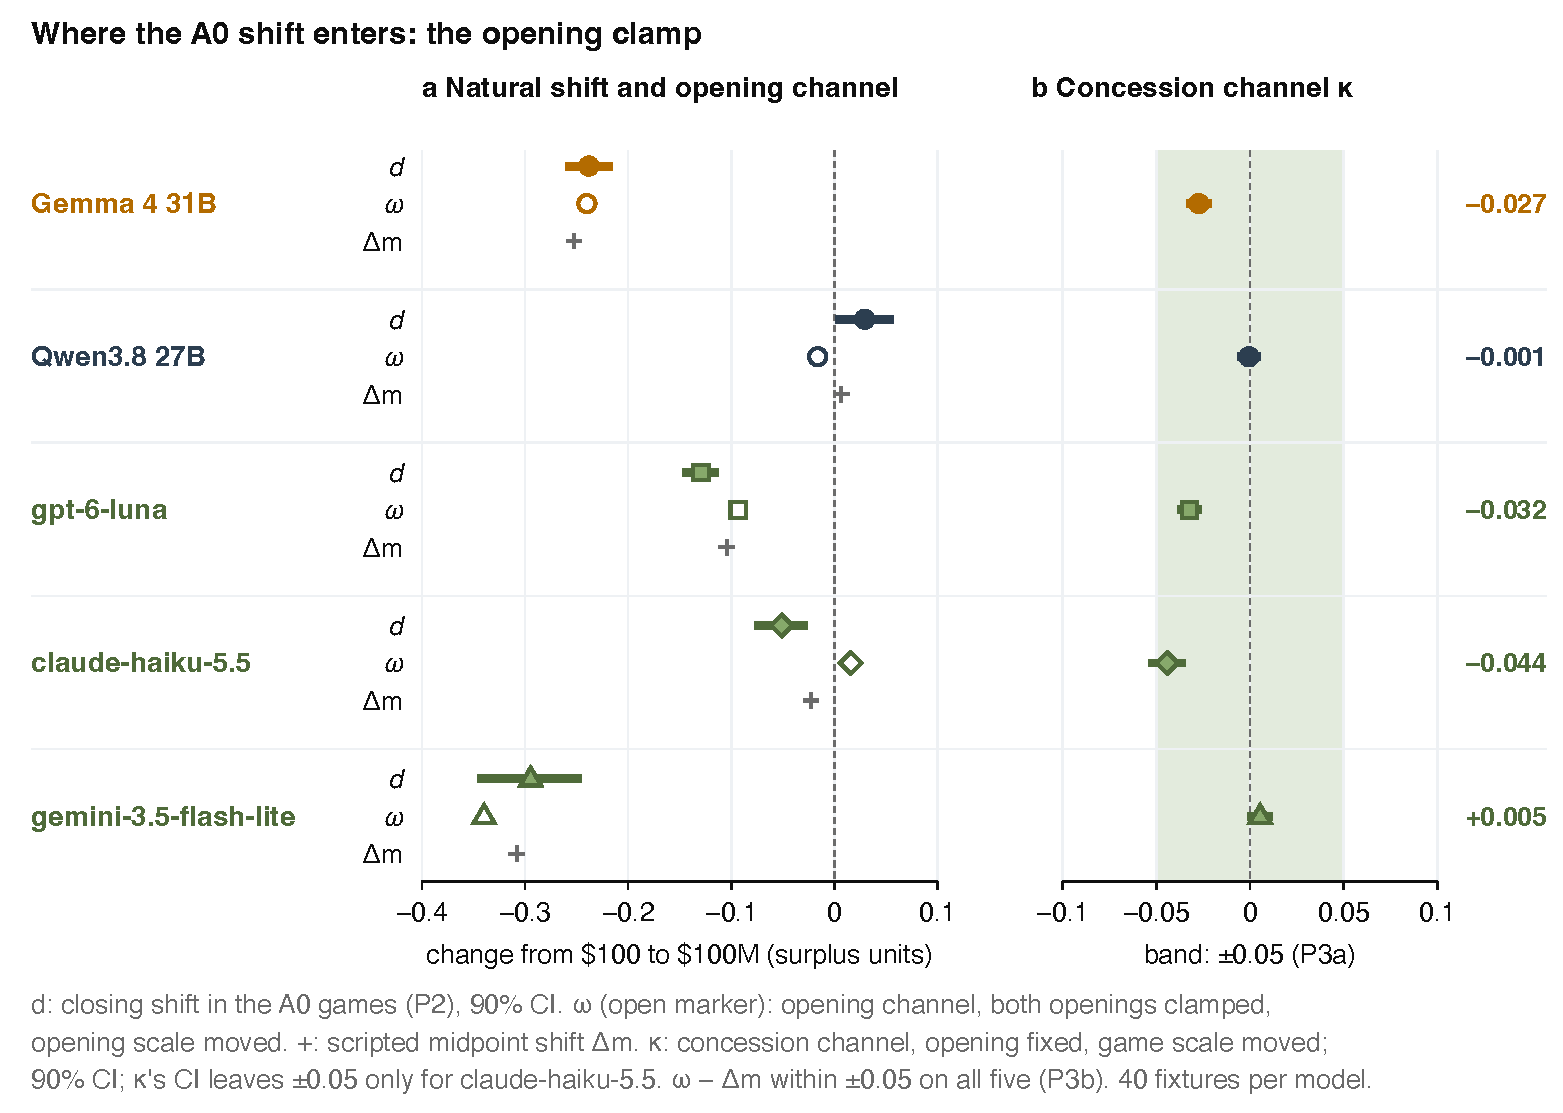
\includegraphics[width=0.95\textwidth]{../manuscript/figures/s3_clamp.pdf}
  \caption{Where the no-appraisal shift enters. (a) Natural closing shift $d$ (90\% CI), opening channel $\omega$ (open marker), and scripted midpoint shift $\Delta m$ (cross). (b) Concession channel $\kappa$ with 90\% CI; band $\pm 0.05$.}
  \label{fig:s3-clamp}
\end{figure}

Holding the openings fixed and changing only the game's scale leaves a concession channel $\kappa$ within $\pm 0.05$ on four models. It is detectably negative on Gemma (\sThreeKappaGemma{}) and Luna (\sThreeKappaLuna{}): with identical openings, deals settle slightly lower at \$100M. On Haiku $\kappa$ is not shown equivalent to zero (\sThreeKappaHaiku{} \sThreeKappaCIHaiku{}; its 90\% CI crosses the margin), so its behaviour at scale is not explained by openings alone; Haiku is also the one model whose natural deals track the first offers' midpoint only weakly (S5: Spearman \sThreeSfiveRhoHaiku{}, against \sThreeSfiveRhoLuna{}--\sThreeSfiveRhoGemma{} for the others).

Scripted openings are not natural ones. At \$100M the scripted cells settle lower than natural games on Qwen (\sThreeSsixHighQwen{}) and Gemini (\sThreeSsixHighGemini{}; S6, both $p < 0.001$; Table~\ref{tab:s3-sec-b}), likely because replacing natural opening messages with a neutral template and clamping mean zone positions interacts with scale. On Gemini, the \$100M offset is roughly a third of the natural shift and differs from the \$100 offset ($-0.058$) by $\sim 0.04$, which bounds the precision of its $\kappa$ and $\omega$ estimates.

\subsection{Boundary conditions from exploratory probes}
\label{sec:res-controls}

Four natural questions arise from Study 3's protocol: whether explicit scale-neutral prompting removes opening modesty, whether integer-dollar discretization or digit strings drive the small-scale gap, whether symmetric self-play masks surplus loss in cross-model play, and how sensitive the split is to zone geometry and framing. While Study 3 holds those factors fixed, the discovery phase executed over 10{,}000 exploratory games on Gemma 4 31B and Qwen3.8 27B (not the API models) that directly probe each boundary condition (Appendix~\ref{app:d10}, Figures~\ref{fig:app-probes}--\ref{fig:app-digits}). We summarize them here, explicitly labeled \emph{exploratory}:

\begin{itemize}
  \item \textbf{Explicit scale-neutral instructions fail (X20--X21, 4{,}320 games).} Appending the explicit instruction \emph{``The size of the numbers does not change what good negotiating looks like. Negotiate exactly as you would if every amount were a thousand times smaller or a thousand times larger''}---as well as tough or cooperative style directives---fails to remove opening shrinkage in either model. Across all four styles, Gemma retains 38--47\% seller opening shrinkage and 18--24\% buyer shrinkage, and Qwen retains 6--13 percentage points of shrinkage. Against a scale-invariant scripted counterpart, Qwen's own surplus share still falls by 0.04--0.14 across every style and role, most steeply when instructed to be tough.
  \item \textbf{Both digits and unit words contribute, even with cents shown (X15--X16, 3{,}600 first moves on Gemma).} Keeping the digits fixed (e.g., ``81'') while changing the unit to millions reproduces 61\% of the full millionfold opening shift ($-8.9$ of $-14.5$ percentage points; negative in 30/30 fixtures), while changing the digit string at fixed stakes accounts for the remaining $-5.6$ points (negative in 28/30 fixtures). Displaying explicit cents (``81.00 dollars'') does not remove the small-scale vs.\ large-scale gap and retains 97\% round-ten seller openings (versus 99\% for plain small-dollar wording and 35--57\% under other wordings); adding a ``\$'' sign changes the both-role gap by only 2--3 points. Combined with Study 3's confirmatory \$100K $\to$ \$100M shifts (S2), this shows that neither whole-dollar discretization nor digit length alone explains the effect.
  \item \textbf{Cross-model asymmetric play confirms surplus transfer (X19, 960 games).} Pairing high-shrinkage Gemma against more scale-stable Qwen tests whether mutual modesty in self-play conceals real surplus loss. When Gemma sells to Qwen, seller share drops by $-0.113$ at $\times 10^6$; in the reverse pairing (Qwen selling to Gemma), the shift is smaller ($-0.042$, non-significant).
  \item \textbf{Zone geometry and realistic redesigns modulate self-play splits (X17, X18, X22, 4{,}920 games).} Narrow off-centre zones induce a significant self-play shift even on Qwen ($-0.12$, 95\% CI [$-0.21, -0.03$]) despite its wide-zone equivalence; business notation attenuates Gemma's self-play shift by 0.03--0.09. Moreover, in a redesigned game combining off-centre ranges, business notation, and cents (X17), Gemma's self-play split shift vanished ($+0.027$, 95\% CI [$-0.036, +0.088$] after excluding 68 comma-truncated games), even though both opening gaps still fell (16.5 points for sellers, 9.2 for buyers) and seller losses against a scale-invariant bot persisted ($-0.258$ [$-0.318, -0.199$]).
\end{itemize}

\subsection{Repeatability}
\label{sec:res-repeatability}

Every primary statistic was estimated separately in the two sessions (S7), which used disjoint sample indices (samples 1--2 vs.\ 3--4, hence different random seeds rather than repeated runs of identical seeds). Five of 25 session differences have 95\% CIs excluding zero, the largest being Qwen's shift under the appraisal ($+0.103$ in session 1, $+0.050$ in session 2). Applying the registered rules to each session separately (not a registered comparison), two verdicts differ: Qwen's equivalence under the appraisal fails in session 1 and passes in session 2, and Haiku's P3b passes in session 1 and fails in session 2. The pooled values in Table~\ref{tab:s3-primary} are the registered primary results, though Qwen's near-margin A1 shift warrants caution.

\subsection{Post-Study 3 robustness: thinking enabled and \$1{,}000 anchor (Addendum D)}
\label{sec:res-addendum-d}

To directly test the two largest protocol-level confounders---thinking disabled and the whole-dollar \$100 baseline---we froze a follow-up preregistration (Addendum D; Appendix~\ref{app:addendum-d}) and ran 960 new games on \texttt{gemini-3.5-flash-lite} across Study 3's exact 40 fixtures (G01--G40, $k = 2$ per cell; Table~\ref{tab:addendum-d}):
\begin{itemize}
  \item \textbf{Enabling native thinking attenuates but does not remove the scale shift (Block D1, \addDOneGames{} Gemini games + 160 open-weight games).} On Gemini with native chain-of-thought enabled (\texttt{thinkingBudget=1024}, averaging \addDOneMeanThought{} thinking tokens per call), agreement reached 640/640 with \addDOneOutside{} outside-zone deals (down from 120 in Study 3). Under A0, enabling thinking attenuated the closing shift by \addDOneAzeroDelta{} ($p =$ \addDOneAzeroDeltaP{}), yet a large, highly significant scale shift persisted ($d =$ \addDOneAzeroD{}, 90\% CI \addDOneAzeroDCI{}, $p$ \addDOneAzeroDP{}) alongside strong opening modesty ($h =$ \addDOneAzeroH{}, $p < 0.001$). Under A1, the sign reversal likewise persisted ($d =$ \addDOneAoneD{}, 90\% CI \addDOneAoneDCI{}, $p$ \addDOneAoneDP{}; P1 $I =$ \addDOnePoneI{}). On open-weight pods (capped at 45 min, \addDOneGemmaGames{} games per model), Gemma 4 31B with thinking enabled still showed a strong A0 shift ($d =$ \addDOneGemmaD{}, 90\% CI \addDOneGemmaDCI{}, $p$ \addDOneGemmaDP{}, $n = \addDOneGemmaNFx{}$ paired fixtures; $h =$ \addDOneGemmaH{}), while Qwen3.8 27B frequently exceeded the 4{,}096-token budget mid-thought (62/80 truncations) yet still exhibited opening modesty on paired first moves ($h =$ \addDOneQwenH{}, $p =$ \addDOneQwenHP{}).
  \item \textbf{3-model cross-play confirms asymmetric surplus transfer (Block D2, 200 A0 games across G01--G40).} Pairing \{Gemma 4 31B, Qwen3.8 27B, Gemini\} across all six directed off-diagonal matchups (198/200 agreements, 0 forfeits; Table~\ref{tab:addendum-d2}, exploratory due to pod-cap truncation) confirmed the predicted asymmetry: high-shrinkage sellers lost 16--30 points against Qwen (Gemma $\to$ Qwen $-0.296$; Gemini $\to$ Qwen $-0.160$), whereas Qwen selling to Gemini \emph{gained} $+0.139$ at \$100M (and Qwen $\to$ Gemma stayed near zero at $-0.032$).
  \item \textbf{Replacing \$100 with \$1{,}000 confirms a large continuous-scale shift alongside a small-integer component (Block D3, \addDThreeGames{} games).} Moving the low-scale anchor to \$1{,}000 (where \$1 is $< 0.5\%$ of the zone) still yielded a large negative A0 closing shift to \$100M ($d =$ \addDThreeD{}, 90\% CI \addDThreeDCI{}, $p$ \addDThreeDP{}). Comparing against Study 3's $\$100\text{M} - \$100$ shift ($\Delta =$ \addDThreeDelta{}, 90\% CI \addDThreeDeltaCI{}) separates the two effects: roughly 43\% of Gemini's full shift arises between \$100 and \$1{,}000, while 57\% ($-0.167$) persists from \$1{,}000 to \$100M where integer discretization is negligible.
\end{itemize}

% Auto-generated from derived/addendum_d/addendum_d.json
\begin{table}[t]
\centering
\caption{Addendum D preregistered robustness checks on \texttt{gemini-3.5-flash-lite} across Study 3's exact 40 fixtures (G01--G40, $k = 2$ per cell). Paired Wilcoxon sign-flip $p$-values (200{,}000 flips) and 90\% fixture-bootstrap CIs. D1 enables native thinking (\texttt{thinkingBudget=1024}, mean 274.9 thinking tokens/call, 640/640 agreements, 0 outside-zone deals). D3 replaces the \$100 baseline with \$1{,}000 (318/320 agreements, 0 forfeits).}
\label{tab:addendum-d}
\footnotesize
\setlength{\tabcolsep}{4pt}
\resizebox{\textwidth}{!}{%
\begin{tabular}{@{}lcccc@{}}
\toprule
Block / Contrast & Games & Estimate [90\% CI] & $p$ & Paired $\Delta$ vs.\ Study 3 \\
\midrule
D1 Thinking-On, A0 closing $d$ (\$100M $-$ \$100) & 320 & $-$0.178 [$-$0.210, $-$0.146] & $< 0.001$ & $+$0.116 ($p$ $0.008$) \\
D1 Thinking-On, A0 opening $h$ (\$100M $-$ \$100) & 320 & $-$0.204 [$-$0.215, $-$0.193] & $< 0.001$ & --- \\
D1 Thinking-On, A1 closing $d$ (\$100M $-$ \$100) & 320 & $+$0.065 [$+$0.046, $+$0.083] & $< 0.001$ & $-$0.036 ($p$ $0.003$) \\
D1 Thinking-On, P1 interaction $I = h(\text{A1}) - h(\text{A0})$ & 640 & $+$0.145 [$+$0.131, $+$0.159] & $< 0.001$ & --- \\
\midrule
D3 \$1{,}000 Anchor, A0 closing $d$ (\$100M $-$ \$1K) & 320 & $-$0.167 [$-$0.236, $-$0.101] & $< 0.001$ & $+$0.127 [$+$0.066, $+$0.188] \\
\bottomrule
\end{tabular}%
}
\end{table}


\section{Inside Gemma: where the appraisal acts, and what the scale signal carries}
\label{sec:interp}

This section reports two exploratory analyses, E5 and E6. Their predictions were written from the discovery-phase results (for E6, also E5's) and committed before each run, and are scored as hits or misses (Tables~\ref{tab:e5-preds} and~\ref{tab:e6-preds}). Methods and full results are in Appendices~\ref{app:e5} and~\ref{app:e6}.

\paragraph{Setup (E5).} We hooked Gemma 4 31B in \texttt{transformers} on Study 3's own first-move prompts (A0 and A1 at \$100 and \$100M), one fixture per distinct limit: 19 seller floors and 18 buyer ceilings (17 usable, as G30's two A0 greedy prices are equal). Sampled openings were within 1.2 points of Study 3's vLLM openings in every cell (Table~\ref{tab:e5-gate}). The readout is the forced opening's log-odds between the two no-appraisal greedy prices at \$100 and \$100M. The main intervention, the ``appraisal swap'', copies one run's residual-stream states on the prompt's final segment and the reply's opening tokens into the other run at \$100M, one layer at a time, and reports the share of the log-odds distance between the two runs that it moves.

\paragraph{The appraisal weakens the scale effect on the opening without removing it.} Under the appraisal, the sellers' forced opening keeps \eFiveGapShare{} of the no-appraisal log-odds gap between scales (E5-1). The no-appraisal scale direction at layer 42 still moves real appraisal openings, by \eFiveSteerAoneLow{}--\eFiveSteerAoneHigh{} of the gap, against \eFiveSteerAzeroLow{}--\eFiveSteerAzeroHigh{} for no-appraisal openings (E5-4). Magnitude is still represented; it has less control over the price.

\paragraph{It takes over at layer 41, on the price-writing tokens (Figure~\ref{fig:s3-e5}).} For sellers, swapping in the appraisal run's states moves \eFiveSwapFortyOne{} at layer 41 and \eFiveSwapFortyTwo{} at layer 42 (E5-2). Earlier layers do not merely fail to help: between layers 30 and 40 the swap moves the opening the wrong way, by up to 35\% (61\% when removing the appraisal). The committed scoring rule (a signed maximum up to layer 39) counts E5-2 as a hit; read as a magnitude bound it would be a miss. At layer 44 the reply's opening tokens carry \eFiveReplyShare{} and the prompt's final segment \eFivePromptShare{} (E5-3). Buyers miss the predicted onset (E5-6): they begin using the appraisal gradually from layer 30, about 40\% by layers 36--40, before the same takeover at layer 41 (buyer shares are less reliable because in the appraisal run at \$100M only \eFiveBuyerProbMass{} of the probability falls on the two readout prices; Appendix~\ref{app:e5}).

\begin{figure}[t]
  \centering
  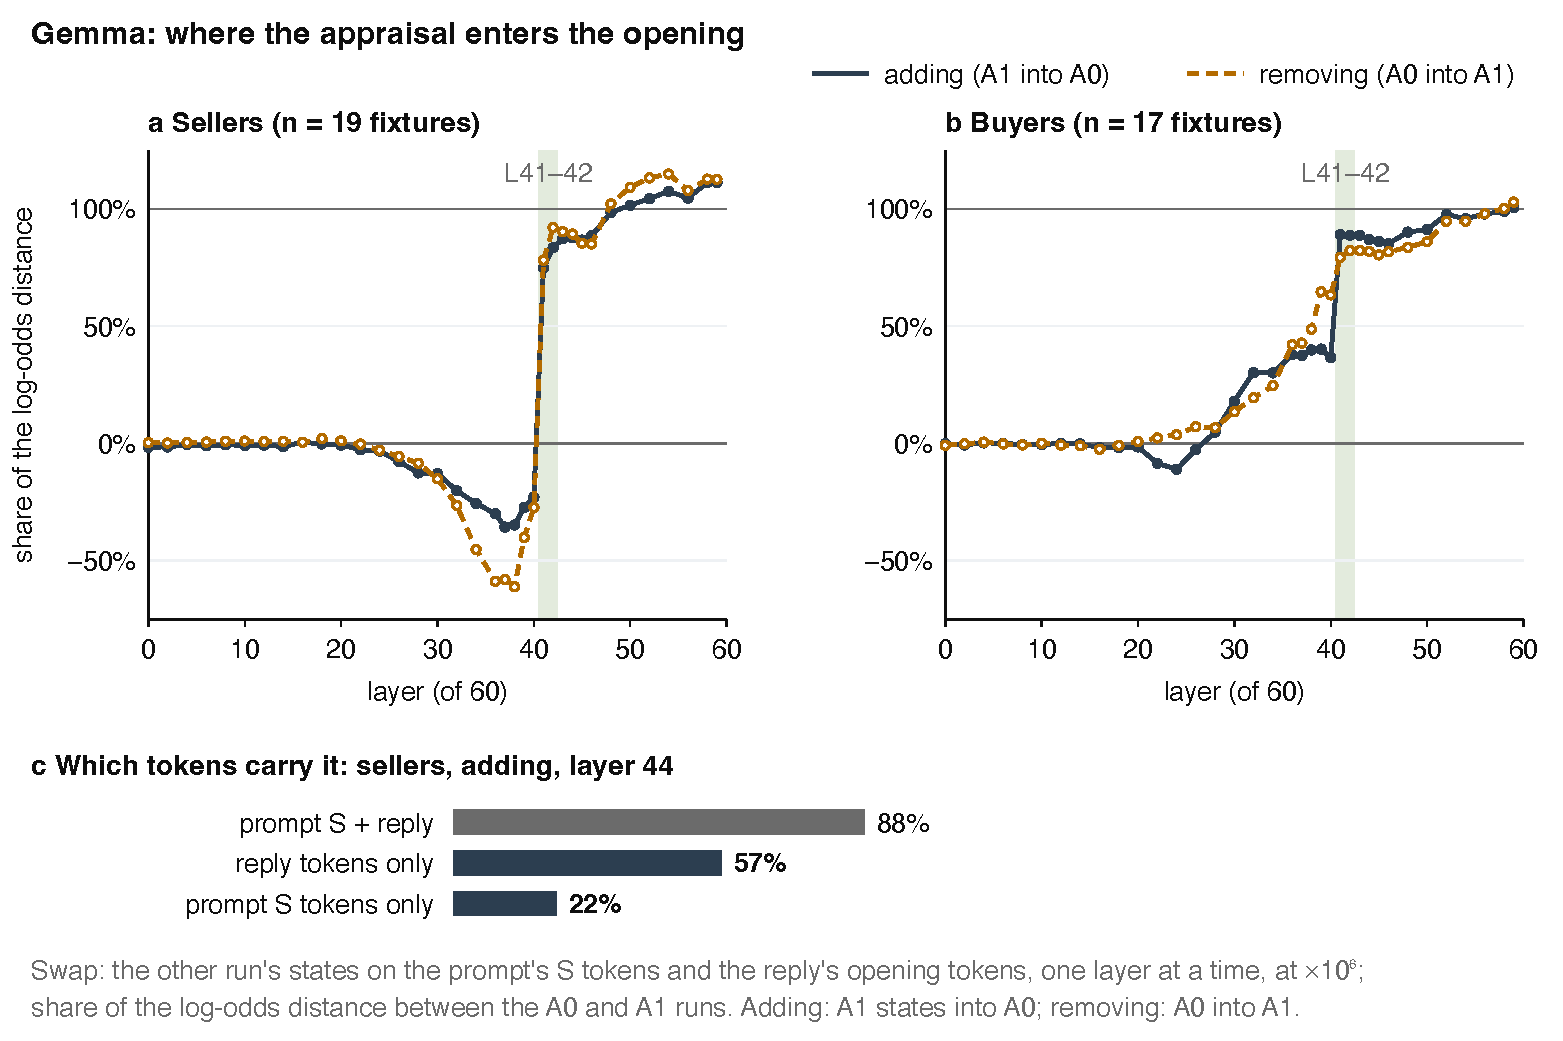
\includegraphics[width=0.95\textwidth]{../manuscript/figures/s3_e5.pdf}
  \caption{Where the appraisal enters Gemma's opening (exploratory). (a) Sellers, 19 floors; (b) buyers, 17 ceilings. Share of the log-odds distance between the no-appraisal and appraisal runs moved by swapping one run's states into the other at one layer, at \$100M; adding (appraisal states into the no-appraisal run) and removing. Band: layers 41--42. (c) Token split at layer 44, sellers, adding.}
  \label{fig:s3-e5}
\end{figure}

\paragraph{Largely the same heads as the scale and range effects.} Ranked on 7 discovery floors, \eFiveHeadOverlap{} of the appraisal's top eight heads (at layers 39--43, four at layer 41) are among the 13 heads that carried the scale and private-range effects in the discovery phase (expected overlap by chance $\approx 0.46$; Table~\ref{tab:e5-heads}). On the 12 held-out floors, patching those eight heads' outputs from the appraisal run into the no-appraisal \$100M run moves the opening log-odds toward the \$100 price on \textbf{12 of 12} floors (mean \eFiveHeldOutMoved{} nats), restoring \textbf{\eFiveHeldOutOwnGapPct{}} of those floors' own A0 scale gap ($+18.69$ nats), whereas eight random heads move \eFiveHeldOutRandMoved{} nats ($\approx 0\%$; Table~\ref{tab:e5-circuit}).\footnote{For pre-commitment transparency, the pre-committed E5-5 held-out ratio (\eFiveHeldOutRatio{}) divided this mean move by the A1 $-$ A0 log-odds distance on the A0-price readout; because that denominator flips sign across floors ($-26.0$ to $+7.1$ nats), the ratio is not a bounded share. We therefore lead with the sign-consistent direct move and own-gap share (computed post hoc) and report both metrics per floor in Appendix~\ref{app:e5} (Table~\ref{tab:e5-circuit}).}

\subsection{Number or stakes? (E6)}
\label{sec:e6}

If the opening shift is a stake effect, the direction that carries it should also move choices where the stakes matter but negotiation does not. If it is a number effect, it should carry the size of the number and little else. E6 tests this in two parts, with ten predictions committed before the run (Table~\ref{tab:e6-preds}).

\paragraph{Gemma reads magnitude the same way in five notations.} We recorded Gemma's states on 360 one-sentence statements of an amount (nine mantissas $\times$ $10^0$ to $10^7$) in five notations: ``3700 dollars'', ``3.7 thousand dollars'', ``\$3.7K'', ``\$3,700'', and ``3700 people''. At the sentence's last token, a magnitude direction fitted on the digit sentences alone reads the log amount of the word and abbreviated sentences at $r = 0.97$ and $0.96$ by layer 20 (Figure~\ref{fig:s3-e6}a; E6-2). This looks computed rather than lexical: at layers 1--2 the same direction reads ``\$3.7K'' at $r \approx 0$ and ``3.7 thousand dollars'' at $0.43$--$0.45$, and the shared code forms between layers 3 and 5 (E6-3). Among MLP neurons, 1{,}640 of 21{,}504 at layer 20 rise or fall with the amount in all four money notations ($|\text{Spearman } \rho| \ge 0.8$), and 609 of them also track head counts (Figure~\ref{fig:s3-e6}b).

\paragraph{Gemma has a stake effect of its own, in risky choices.} Offered a sure amount or a 50\% chance of twice that, or of 2.4 or 3 times that---with option order (\texttt{safeA}/\texttt{safeB}) strictly counterbalanced across all 30 matched pairs---Gemma at \$100 takes the gamble when its expected value is higher (18 of 20). At \$100M it no longer prefers the better gamble: its discrete choices follow the listing order (the first-listed option in 18 of 20), while across the counterbalanced pairs the log-odds of the safe option rise by \eSixRiskNatGap{} nats (E6-5). Thus the log-odds shift moves in the direction people show when payoffs are scaled up \citep{holt2002risk}, although the discrete \$100M choices reflect loss of EV sensitivity and order bias rather than pure risk aversion.

\paragraph{The negotiation's scale direction barely moves it.} We took the direction separating Gemma's \$100M and \$100 seller openings at layer 42 (from E5's 19 fixtures; leave-one-fixture-out on negotiation prompts), added it to the model's turn on other tasks' \$100 prompts, and measured the share of each task's natural $\$100 \to \$100\text{M}$ gap it reproduced (Figure~\ref{fig:s3-e6}c). It moves negotiation openings \eSixNegMove{} of the way, against \eSixNegRand{} for a random vector of the same norm (E6-1), but moves risky choices \eSixRiskMove{} and percentage answers \eSixPctMove{}, far short of the predicted 25\% (non-money control \eSixRiskCtrl{} and \eSixPctCtrl{}; E6-6 and E6-7 missed). It leaves comparisons and sums intact (E6-8). It does make numbers larger: Fermi estimates rise by \eSixFermiPlus{} orders of magnitude at $\alpha = +2$ and fall by \eSixFermiMinus{} at $-2$ (E6-9 missed), driven by three of ten items that jump by two to five orders of magnitude. The control direction does the same ($+0.97$), so this leak is not specific to the negotiation direction. The negotiation direction also overlaps the plain-sentence magnitude direction (cosine \eSixCos{} at layer 42, against about 0.014 by chance; E6-10 missed at its 0.2 threshold).

With E5, this places Gemma's scale effect. Magnitude is read early and the same way in five notations; a late stage at layers 41--44 uses it to set the price, and a competing reference number (the private range or the appraisal) can take over there. The direction that shifts the openings behaves more like a signal of numerical magnitude than of stakes: adding it reproduces \eSixRiskMove{} of Gemma's stake effect in risky choices. In this model the opening shift looks like a number effect applied by the negotiation, not an imported risk preference. This rests on one model, one steering placement, and two layers. Appendix~\ref{app:e6} reports three scoring artefacts in the original E6 run (E6-4 is met trivially at L0, the exponent-tuning count cannot reach its threshold, and isotropic random vectors break short prompts). To verify that the null risk/percentage transfer is not an artefact of a broken random baseline, a follow-up control (\textbf{E6b}, Table~\ref{tab:e6b}) replaced the isotropic Gaussian with a layer-covariance-matched random direction orthogonalized to the 9-dimensional reply/format subspace at layer 42 ($\cos(v_R, \texttt{rand\_cov}) = 0.000$, identical norm $30.39$): \texttt{rand\_cov} preserved \eSixBRiskMass{} valid-option mass on risk and comparison prompts and 100\% parse rate on percentages and sums while moving risky choices by \eSixBRiskShare{} (\eSixBRiskShareOne{} at $\alpha = +1$) and percentages by \eSixBPctShare{}.

\begin{figure}[t]
  \centering
  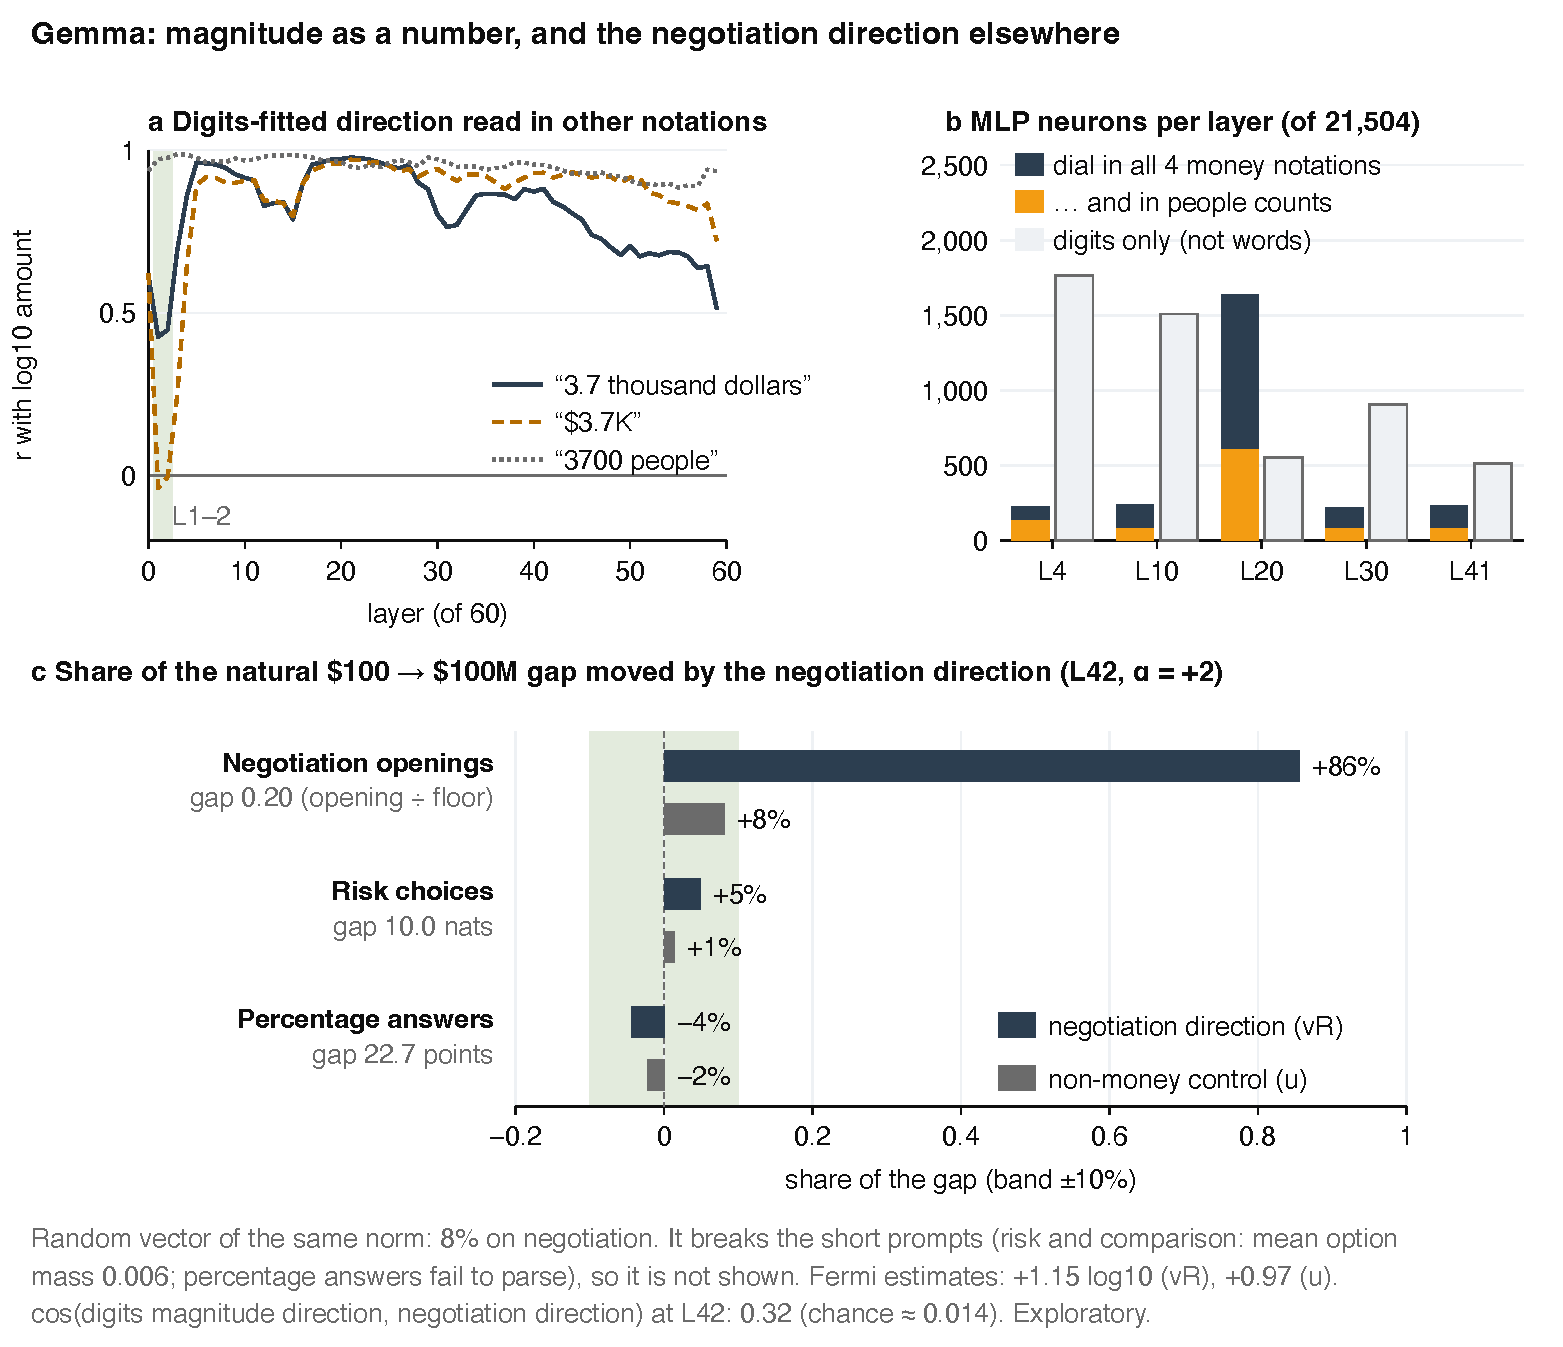
\includegraphics[width=0.95\textwidth]{../manuscript/figures/s3_e6.pdf}
  \caption{Magnitude as a number, and the negotiation direction in other tasks (Gemma, exploratory). (a) Correlation with log amount of the projection onto a magnitude direction fitted on digit sentences, read in three other notations, by layer. (b) MLP neurons whose activation follows the amount ($|\rho| \ge 0.8$) in all four money notations, the subset that also follows head counts, and neurons that follow digits but not words. (c) Share of each task's natural $\$100 \to \$100\text{M}$ gap moved by adding the negotiation scale direction or a non-money control at layer 42, $\alpha = +2$, on \$100 prompts.}
  \label{fig:s3-e6}
\end{figure}

\section{Discussion}
\label{sec:discussion}

\paragraph{What the models comprehend.} The models are not blind to magnitude. Gemma reads amounts on one number line in five notations by layer 5 (Section~\ref{sec:e6}), and its scale signal persists, with less effect on the price, under the appraisal (Section~\ref{sec:interp}). What changes with scale is the opening, and outcomes follow the openings: deals follow the scripted openings on every model, and on the three models whose split moves, the openings account for most of the shift. The departure is therefore a policy that maps larger absolute amounts to more modest relative opening positions, not a failure to read the numbers. It resembles the stake effects people show, and Gemma has one in risky choices; but in Gemma the direction that shifts the openings barely moves those choices, and behaves more like a signal of numerical magnitude.

\paragraph{Whose stake preferences?} A person selling a \$100M asset may reasonably be more cautious than one selling a \$100 one. An agent acting for that person has not been told to be---and even when explicitly instructed to be scale-neutral, opening shrinkage persists (Section~\ref{sec:res-controls}). Caution alone also cannot move a self-play split: when both sides share the same utility over their gains, the Nash solution divides the surplus equally at every scale, however risk averse they are \citep{nash1950bargaining, kihlstrom1981risk}. The closing shifts therefore need an asymmetry between roles, and Study 3 shows one. Without the appraisal, from \$100 to \$100M the sellers' opening gap narrows two to three and a half times as much as the buyers' on the three models whose split shifts (Gemma 0.21 against 0.11, Luna 0.16 against 0.04, Gemini 0.34 against 0.15). Haiku shows a similar imbalance (0.15 against 0.06) with a smaller shift (\sThreeAzeroHaiku{}), and its deals track the opening midpoint least (S5), so the imbalance alone does not set the size of the shift. For deployment the question is less whether a model is rational than whether it brings in a preference its principal did not state.

\paragraph{Self-play invariance is not robustness.} Qwen's and Haiku's no-appraisal splits meet equivalence, yet their openers still move toward their limits at scale. In self-play, modesty on both sides can offset in the split; against a counterpart that does not share it, the same policy loses surplus, as confirmed in our exploratory cross-play (X19: Gemma selling to Qwen drops by $-0.113$; Addendum D2 3-model cross-play: Gemma $\to$ Qwen $-0.296$, Gemini $\to$ Qwen $-0.160$, whereas Qwen $\to$ Gemini gains $+0.139$; Sections~\ref{sec:res-controls} and~\ref{sec:res-addendum-d}) and scripted-bot probes. An evaluation that checks only outcomes at one scale, or only self-play at several, would miss this.

\paragraph{A reference number is an anchor, not a cure.} The appraisal's effect is model-specific. It anchors every model's deals to its position in the zone, but what it does to the openings at scale differs: it holds Gemma's and Qwen's sellers' openings nearly level, draws Gemini's sellers to just below the appraisal, and leaves Haiku's sellers to collapse further. For Gemma's sellers it acts at the same narrow stage as the scale effect itself, through largely the same heads, on the tokens that write the price. That suggests a single late stage at which a number in context, a limit or an appraisal, can set the price. This is one model and an exploratory analysis; it describes where the intervention acts, not a semantic explanation of the model's numerical representation.

\paragraph{For evaluation.} Agent evaluations that use one price range should report openings as well as outcomes and test at more than one scale. Our design (fixed geometry, shared seeds, an opening clamp) is cheap: Study 3 cost about \$17 in API fees and \$11 in GPU time.

\section{Limitations}
\label{sec:limitations}

The five models are not a representative sample; their precisions and sampling settings differ, so cross-model comparisons are descriptive. All confirmatory Study 3 games use one prompt family and one single-issue task, in self-play, with thinking off or minimised (Addendum D in Section~\ref{sec:res-addendum-d} extends this to thinking-on across three models, 3-model cross-play, and a \$1{,}000 anchor, though open-weight D1/D2 runs were truncated by the 45-minute pod cap and Qwen truncated 62/80 thinking turns at 4{,}096 tokens). Prices are whole dollars, which discretises the \$100 scale (though exploratory cents probes in Section~\ref{sec:res-controls}, Study 3's S2 \$100K $\to$ \$100M shifts, and Addendum D3's \$1{,}000 anchor check all confirm large continuous-scale effects). Each scale change also changes the digit strings; the exploratory digits probes (Section~\ref{sec:res-controls}, Appendix~\ref{app:d10}) attribute part of the opening effect to the digits rather than the stakes. The appraisal is one wording at one place in the prompt.

The hypotheses were informed by earlier data on the same models, so Study 3 confirms them on new bargains, not on new models. An interim look at Gemma and Qwen preceded the second API session; it was logged and changed nothing, but it is a departure from a fully blind sequence. Games with scripted openings settle lower than natural games on Qwen and Gemini at \$100M (S6). API results concern the dated versions returned on 14--15 October 2026. The registration is a local hashed commit, not lodged with an external registry, so its timing rests on the local history and the session manifests (Appendix~\ref{app:reg}).

The mechanistic analysis covers one model, first moves only, and the prompts of 19 seller floors and 18 buyer ceilings, using a forced-opening readout that does not lie on the axis of the appraisal's own openings; that is why the pre-committed E5-5 ratio is uninterpretable as a share. Its predictions were committed, but it is exploratory. E6 adds one steering placement (the model's turn) at two layers; a stake signal elsewhere in the network, or one read from the prompt itself, is not excluded. Stake effects outside negotiation were measured on Gemma only.

\section*{Broader Impact and Reproducibility Statement}

LLM agents deployed in commercial negotiation, procurement, or automated trading may inherit unrequested stake-dependent opening modesty that shifts surplus unevenly across price regimes and counterparties. Evaluating such systems at small benchmark prices does not certify behaviour at large financial stakes.

The registration, hashed inputs (37 frozen files), data-access log, analysis code, and figure and table generators are included in \repoRef{} (Appendix~\ref{app:reg}). Raw call and game records, session manifests, and derived files are archived with cryptographic hashes in each run summary; every game record replays deterministically from its raw calls. The E5 and E6 prediction files were committed before their runs, and their hashes are recorded in the run manifests. AI tools assisted with code, analysis, figures, and checking prose; the authors retain full responsibility for the final text, factual verification, and interpretation \citep{arxiv2025aipolicy}.

\bibliography{references}
\bibliographystyle{tmlr}

\ifincludeappendix
\clearpage
\appendix
\section{Registration, freeze, data access, and deviations}
\label{app:reg}

\begin{itemize}
  \item \textbf{Registration.} \texttt{prereg/study3/PREREGISTRATION.md} v3, frozen with \texttt{prereg/study3/inputs.sha256} (37 files) in commit \texttt{c8feea1} on 14 October 2026, before any registered game. It was not lodged with any external registry. The frozen document still carries its draft status line (``NOT registered, NOT frozen'') and its plan to record an external registry's timestamp before any game; the freeze commit and the hash check were carried out as written, while the external timestamp was not. The freeze order rests on the local git history (\texttt{c8feea1} at 17:28 MDT, 23:28 UTC) and on the six session manifests, which record the commit each session ran from (\texttt{c8feea1}; for API session 2, \texttt{c2292c1}, which adds only the data-access log) and the hash of every frozen file. The first registered call was sent at 23:54 UTC, 25 minutes after the freeze commit.
  \item \textbf{Decisions before the freeze.} (1) Scripted openings in zone units rather than own-limit gaps, set on 13 October before any game, because transplanted gaps made some scripted pairs cross. (2) Trailing text after the first JSON object is ignored and flagged (14 October, after the first API pilot, which was rerun under it). Luna had \sThreeTrailingLuna{} such replies; no other model had any.
  \item \textbf{Data access.} Logged in \texttt{prereg/study3/DATA\_ACCESS.md}, each entry committed before the look: an interim look at Gemma and Qwen (commit \texttt{c2292c1}) before the second API session, and the single registered analysis of all five models (commit \texttt{8a3167d}).
  \item \textbf{Run incident.} API session 2 stalled when the host machine slept after 1{,}266 games. It was resumed from the same commit; no finished game was replayed and no attempt was voided.
  \item \textbf{Quality.} Counts by model are in Table~\ref{tab:s3-quality}. Luna had \sThreeForfeitsLuna{} forfeits and \sThreeTimeoutsLuna{} timeouts. All three API models had 0 refusals, 0 reasoning tokens, and 0 reasoning text (Gemini included). Returned versions were unchanged across sessions: \texttt{openai/gpt-6-luna-20260922}, \texttt{anthropic/claude-haiku-5.5-20261007}, and \texttt{google/gemini-3.5-flash-lite-20260721}.
  \item \textbf{Cost.} API fees, as OpenRouter reported them, were \$16.96 for the two registered sessions and \$0.56 for the two format pilots. GPU time for Study 3 was about \$10.90 including its pilots, and for E5 and E6 about \$1.62 and \$0.58 (launcher estimates, not billing records).
\end{itemize}

\section{Full Study 3 results}
\label{app:study3-full}

Table~\ref{tab:s3-quality} gives game outcomes and data quality by model. Outside-zone agreements (retained unclipped, as registered) broke down by cell as follows: \textbf{Gemini} (120/3{,}200): A0 9/320 at \$100, 8 at \$100K, 20 at \$100M; A1 38 at \$100, 7 at \$100K, 4 at \$100M; clamp 24 (\texttt{x1e2-o1e2}), 7 (\texttt{x1e2-o1e8}), 3 (\texttt{x1e8-o1e2}), 0 (\texttt{x1e8-o1e8}). \textbf{Haiku} (77/3{,}200): A0 7 at \$100, 9 at \$100K, 26 at \$100M; A1 1 at \$100, 0 at \$100K, 2 at \$100M; clamp 4, 6, 14, 8. \textbf{Qwen} (20/3{,}200): A0 6 at \$100, 12 at \$100M; A1 2 at \$100. Gemma and Luna had zero. The registered secondaries are in Table~\ref{tab:s3-sec-a} (S1--S4), Table~\ref{tab:s3-sec-b} (S5--S9), and Table~\ref{tab:s3-sec-c} (the S3 contrasts not shown before, S8's comparison of A1 with Study 1, and S9's check of whether the A1 shift varies with the appraisal's position). Together with Table~\ref{tab:s3-primary}, these report every registered test.

% Auto-generated from derived/study3/study3.json
\begin{table}[t]
\centering
\caption{Study 3 game outcomes and data quality by model across all ten cells and both sessions. No model had a refusal, a reasoning token, or reasoning text, and no registered quality flag was raised. Agreements outside the zone are retained and scored unclipped, as registered.}
\label{tab:s3-quality}
\footnotesize
\setlength{\tabcolsep}{4.5pt}
\begin{tabular}{@{}lrrrrrrrr@{}}
\toprule
Model & Games & Agreements & Walkaways & Timeout & Forfeits & Outside zone & Trailing text & Mean msgs \\
\midrule
Gemma 4 31B & 3,200 & 3,199 & 1 & 0 & 0 & 0 & 0 & 8.2 \\
Qwen3.8 27B & 3,200 & 3,191 & 9 & 0 & 0 & 20 & 0 & 6.8 \\
gpt-6-luna & 3,200 & 3,130 & 12 & 23 & 35 & 0 & 616 & 14.9 \\
claude-haiku-5.5 & 3,200 & 3,183 & 17 & 0 & 0 & 77 & 0 & 8.0 \\
gemini-3.5-flash-lite & 3,200 & 3,189 & 11 & 0 & 0 & 120 & 0 & 6.7 \\
\bottomrule
\end{tabular}
\end{table}

% Auto-generated from derived/study3/study3.json
\begin{table}[t]
\centering
\caption{Study 3 registered secondaries S1--S4. S1: change in opener's first-offer gap from own limit, \$100M $-$ \$100 [95\% CI; S1 A1 90\% CI]; HA predicts $h(\text{A0}) < 0$ (one-sided, Holm across models). S2: closing shift between adjacent scales (top: A0; bottom: A1; Holm within model). S3: all-game seller utility (A0). S4: opener's advantage change (top: A0; bottom: A1; Holm across models).}
\label{tab:s3-sec-a}
\scriptsize
\setlength{\tabcolsep}{3.5pt}
\resizebox{\textwidth}{!}{%
\begin{tabular}{@{}lcccccc@{}}
\toprule
Model & S1 $h(\text{A0})$ & S1 $h(\text{A1})$, $\pm 0.03$ & S2 \$100K$-$\$100 & S2 \$100M$-$\$100K & S3 util.\ (A0) & S4 HB (A0/A1) \\
\midrule
Gemma 4 31B & \makecell{$-$0.156 ($< 0.001$) \\{} [$-$0.171, $-$0.143]} & \makecell{$-$0.042 (not equiv.) \\{} [$-$0.049, $-$0.037]} & \makecell{A0: $-$0.129 ($< 0.001$) \\{} A1: $-$0.019 ($0.131$)} & \makecell{A0: $-$0.109 ($< 0.001$) \\{} A1: $+$0.021 ($0.032$)} & \makecell{$-$0.239 \\{} ($< 0.001$)} & \makecell{A0: $-$0.141 ($< 0.001$) \\{} A1: $+$0.004 ($0.682$)} \\
\addlinespace[2pt]
Qwen3.8 27B & \makecell{$-$0.117 ($< 0.001$) \\{} [$-$0.130, $-$0.104]} & \makecell{$-$0.016 (equiv.) \\{} [$-$0.022, $-$0.010]} & \makecell{A0: $+$0.037 ($0.083$) \\{} A1: $+$0.066 ($< 0.001$)} & \makecell{A0: $-$0.007 ($1.000$) \\{} A1: $+$0.011 ($0.630$)} & \makecell{$+$0.031 \\{} ($0.630$)} & \makecell{A0: $-$0.244 ($< 0.001$) \\{} A1: $+$0.037 ($0.207$)} \\
\addlinespace[2pt]
gpt-6-luna & \makecell{$-$0.101 ($< 0.001$) \\{} [$-$0.115, $-$0.086]} & \makecell{$-$0.053 (not equiv.) \\{} [$-$0.059, $-$0.048]} & \makecell{A0: $-$0.079 ($< 0.001$) \\{} A1: $-$0.035 ($0.006$)} & \makecell{A0: $-$0.050 ($< 0.001$) \\{} A1: $+$0.005 ($0.577$)} & \makecell{$-$0.133 \\{} ($< 0.001$)} & \makecell{A0: $-$0.030 ($0.483$) \\{} A1: $-$0.134 ($< 0.001$)} \\
\addlinespace[2pt]
claude-haiku-5.5 & \makecell{$-$0.105 ($< 0.001$) \\{} [$-$0.132, $-$0.081]} & \makecell{$-$0.125 (not equiv.) \\{} [$-$0.139, $-$0.112]} & \makecell{A0: $-$0.019 ($1.000$) \\{} A1: $-$0.067 ($< 0.001$)} & \makecell{A0: $-$0.033 ($0.110$) \\{} A1: $-$0.046 ($< 0.001$)} & \makecell{$-$0.051 \\{} ($0.066$)} & \makecell{A0: $+$0.074 ($0.483$) \\{} A1: $-$0.152 ($< 0.001$)} \\
\addlinespace[2pt]
gemini-3.5-flash-lite & \makecell{$-$0.247 ($< 0.001$) \\{} [$-$0.269, $-$0.223]} & \makecell{$-$0.052 (not equiv.) \\{} [$-$0.056, $-$0.049]} & \makecell{A0: $-$0.213 ($< 0.001$) \\{} A1: $+$0.067 ($< 0.001$)} & \makecell{A0: $-$0.082 ($< 0.001$) \\{} A1: $+$0.033 ($< 0.001$)} & \makecell{$-$0.295 \\{} ($< 0.001$)} & \makecell{A0: $-$0.297 ($0.002$) \\{} A1: $-$0.104 ($< 0.001$)} \\
\addlinespace[2pt]
\bottomrule
\end{tabular}%
}
\end{table}

% Auto-generated from derived/study3/study3.json
\begin{table}[t]
\centering
\caption{Study 3 registered secondaries S5--S9. S5: natural A0 deal position minus first offers' midpoint (calibration, 90\% CI) and Spearman tracking (20{,}000 permutations). S6: diagonal clamp cells minus natural A0 games. S8: A0 shift in Study 2 or Addendum C vs Study 3 (unpaired 95\% CI). S9: Spearman correlation between appraisal position in zone and A1 seller share. S7 primary statistics with session-1 vs session-2 paired 95\% CI excluding zero: Gemma 4 31B \texttt{P2\_d\_A1} ($+$0.010 $\to$ $-$0.007); Qwen3.8 27B \texttt{P2\_d\_A1} ($+$0.103 $\to$ $+$0.050); Qwen3.8 27B \texttt{P3b\_omega\_minus\_dm} ($-$0.029 $\to$ $-$0.017); gemini-3.5-flash-lite \texttt{P2\_d\_A1} ($+$0.085 $\to$ $+$0.115); gemini-3.5-flash-lite \texttt{P3a\_kappa} ($-$0.002 $\to$ $+$0.013).}
\label{tab:s3-sec-b}
\scriptsize
\setlength{\tabcolsep}{4pt}
\resizebox{\textwidth}{!}{%
\begin{tabular}{@{}lccccc@{}}
\toprule
Model & S5 cal.\ HM1 ($\pm 0.05$) & S5 track $\rho$ & S6 artefact & S8 A0 vs earlier & S9 $\rho$ (\$100/\$100M) \\
\midrule
Gemma 4 31B & \makecell{$-$0.030 (equiv.) \\{} [$-$0.042, $-$0.017]} & \makecell{0.85 \\{} ($< 0.001$)} & \makecell{\$100: $-$0.009 ($0.611$) \\{} \$100M: $-$0.039 ($0.055$)} & \makecell{$-$0.256 $\to$ $-$0.238 \\{} [$-$0.035, $+$0.067]} & 0.98 / 0.97 \\
\addlinespace[2pt]
Qwen3.8 27B & \makecell{$-$0.033 (not equiv.) \\{} [$-$0.052, $-$0.017]} & \makecell{0.83 \\{} ($< 0.001$)} & \makecell{\$100: $-$0.022 ($0.167$) \\{} \$100M: $-$0.069 ($< 0.001$)} & \makecell{$+$0.009 $\to$ $+$0.029 \\{} [$-$0.094, $+$0.125]} & 0.93 / 0.93 \\
\addlinespace[2pt]
gpt-6-luna & \makecell{$-$0.014 (equiv.) \\{} [$-$0.027, $+$0.001]} & \makecell{0.84 \\{} ($< 0.001$)} & \makecell{\$100: $-$0.006 ($0.635$) \\{} \$100M: $-$0.002 ($0.796$)} & \makecell{$-$0.116 $\to$ $-$0.129 \\{} [$-$0.046, $+$0.019]} & 0.89 / 0.93 \\
\addlinespace[2pt]
claude-haiku-5.5 & \makecell{$+$0.019 (not equiv.) \\{} [$-$0.019, $+$0.060]} & \makecell{0.37 \\{} ($0.011$)} & \makecell{\$100: $-$0.021 ($0.237$) \\{} \$100M: $+$0.002 ($0.883$)} & \makecell{$+$0.006 $\to$ $-$0.051 \\{} [$-$0.099, $-$0.017]} & 0.83 / 0.82 \\
\addlinespace[2pt]
gemini-3.5-flash-lite & \makecell{$-$0.010 (equiv.) \\{} [$-$0.039, $+$0.021]} & \makecell{0.83 \\{} ($< 0.001$)} & \makecell{\$100: $-$0.058 ($0.084$) \\{} \$100M: $-$0.097 ($< 0.001$)} & \makecell{$-$0.304 $\to$ $-$0.295 \\{} [$-$0.084, $+$0.102]} & 0.75 / 0.93 \\
\addlinespace[2pt]
\bottomrule
\end{tabular}%
}
\end{table}

% Auto-generated from derived/study3/study3.json
\begin{table}[t]
\centering
\caption{Remaining Study 3 registered secondaries (S3 agreement rate, coarse-grid prices, A1 seller utility; S8 A1 vs Study 1 on Qwen; S9 appraisal position vs A1 shift). All contrasts are \$100M $-$ \$100 fixture means; S3 $p$-values are two-sided Wilcoxon, Holm within model over the ten S2/S3 contrasts.}
\label{tab:s3-sec-c}
\scriptsize
\setlength{\tabcolsep}{4pt}
\resizebox{\textwidth}{!}{%
\begin{tabular}{@{}lccccc@{}}
\toprule
Model & S3 agr.\ rate & S3 coarse-grid price & S3 util.\ (A1) & S8 A1 vs Study 1 & S9 $\rho$ (A1 shift) \\
\midrule
Gemma 4 31B & \makecell{A0: $-$0.003 ($1.000$) \\{} A1: $+$0.000 ($1.000$)} & \makecell{A0: $-$0.237 ($< 0.001$) \\{} A1: $+$0.002 ($1.000$)} & \makecell{$+$0.002 \\{} ($1.000$)} & --- & $+$0.51 \\
\addlinespace[2pt]
Qwen3.8 27B & \makecell{A0: $+$0.000 ($1.000$) \\{} A1: $+$0.000 ($1.000$)} & \makecell{A0: $+$0.030 ($0.630$) \\{} A1: $+$0.076 ($< 0.001$)} & \makecell{$+$0.077 \\{} ($< 0.001$)} & \makecell{$-$0.032 $\to$ $+$0.077 \\{} diff $+$0.109 [$+$0.061, $+$0.157]} & $+$0.03 \\
\addlinespace[2pt]
gpt-6-luna & \makecell{A0: $-$0.006 ($0.794$) \\{} A1: $-$0.022 ($0.430$)} & \makecell{A0: $-$0.128 ($< 0.001$) \\{} A1: $-$0.029 ($0.006$)} & \makecell{$-$0.041 \\{} ($0.006$)} & --- & $+$0.56 \\
\addlinespace[2pt]
claude-haiku-5.5 & \makecell{A0: $+$0.000 ($1.000$) \\{} A1: $+$0.003 ($1.000$)} & \makecell{A0: $-$0.052 ($0.039$) \\{} A1: $-$0.114 ($< 0.001$)} & \makecell{$-$0.110 \\{} ($< 0.001$)} & --- & $+$0.07 \\
\addlinespace[2pt]
gemini-3.5-flash-lite & \makecell{A0: $-$0.009 ($0.250$) \\{} A1: $+$0.013 ($0.248$)} & \makecell{A0: $-$0.294 ($< 0.001$) \\{} A1: $+$0.101 ($< 0.001$)} & \makecell{$+$0.100 \\{} ($< 0.001$)} & --- & $+$0.40 \\
\addlinespace[2pt]
\bottomrule
\end{tabular}%
}
\end{table}

\FloatBarrier

\section{Protocol details}
\label{app:protocol}

\paragraph{Engine, replies, and validation.} Every game runs on the discovery phase's engine (\texttt{scripts/game\_engine.py}, unchanged); Study 3's own code adds the cells, the scripted openings, the seeds, the request bodies, and the audit (\texttt{scripts/study3.py}). Each call is rebuilt from the system message, the side's own limit, and the public history, in which the other side sees only action, price, and message. A game has at most 16 messages. A reply is capped at 1{,}024 output tokens and must be one JSON object with an action (\texttt{OFFER}, \texttt{ACCEPT}, or \texttt{WALKAWAY}), a price (a whole number of dollars for an \texttt{OFFER}, \texttt{null} otherwise), and a message of at most 500 characters. Every arm gets the same response schema (Addendum C's: that of Studies 1--2 without the \texttt{minimum} and \texttt{maxLength} keywords, which are checked client-side instead) and the same client-side validation. An invalid reply forfeits the game and is never repaired, with one exception set before the freeze: text after the first complete JSON object is ignored and flagged.

\paragraph{Scripted openings.} In the clamp cells the first two messages are written into the public history from the frozen positions in Table~\ref{tab:s3-clamp}: $\text{scripted price} = F + x(C - F)$, rounded half up to a multiple of $V/100$. One neutral template per role is used at every scale and cell, and the history line has the same form as a model's move. No request is sent for messages 1 and 2; the model plays both sides from message 3.

\paragraph{Seeds, order, concurrency, and audit.} A call's seed is the first eight hexadecimal digits of the SHA-256 of \texttt{scale-invariance/study3/v1|fixture|opener|sample|message|attempt}, masked to 31 bits. Scale, appraisal, and clamp cell are not inputs, so every within-fixture contrast shares seeds. Seeds are sent to vLLM, OpenAI, and Google, not to Anthropic. Each model ran two sessions (samples 1--2, then 3--4) on separate GPU pods or separate days, interleaving every core and clamp cell in one fixed shuffle (concurrency 16 on vLLM, 8 on API). Calls, games, and events are hash-chained records; after each session a replay audit re-derived scripted moves, rebuilt every request byte for byte, and re-scored every game from its raw calls. All six sessions passed.

\paragraph{Fixtures and prompts.} G01--G40 come from \texttt{scale-invariance/fixtures/study3-v1} through \texttt{scripts/make\_fixtures.py}, with floors at whole percentages from 75 to 95 and ceilings from 105 to 125 of $V$. The appraisal's position in the zone, $(V - F)/(C - F)$, runs from 0.21 to 0.79 (median 0.48). Table~\ref{tab:s3-arms} lists all five model arms and settings. Prompt templates are reproduced verbatim below.

% Auto-generated from data/runs/s3-*/run_manifest.json
\begin{table}[t]
\centering
\caption{Study 3 model arms and settings from the six session manifests (identical across both sessions of each model). Every arm uses at most 16 messages, 500 characters per message, and 1{,}024 output tokens per reply.}
\label{tab:s3-arms}
\scriptsize
\setlength{\tabcolsep}{3.5pt}
\resizebox{\textwidth}{!}{%
\begin{tabular}{@{}llllllr@{}}
\toprule
Model & Backend & Weights or returned version & Sampling & Thinking & Seed & Conc. \\
\midrule
Gemma 4 31B & vLLM 0.30.0 & \texttt{google/gemma-4-31B-it} @ \texttt{842da37} & temp 1.0, top-$p$ 0.95, top-$k$ 64 & off & yes & 16 \\
Qwen3.8 27B & vLLM 0.30.0 & \texttt{Qwen/Qwen3.8-27B-FP8} @ \texttt{017b9c7} & temp 0.7, top-$p$ 0.8, top-$k$ 20 & off & yes & 16 \\
gpt-6-luna & OpenRouter (OpenAI) & \texttt{openai/gpt-6-luna-20260922} & vendor defaults & effort ``none'' & yes & 8 \\
claude-haiku-5.5 & OpenRouter (Anthropic) & \texttt{anthropic/claude-haiku-5.5-20261007} & vendor defaults & disabled & no & 8 \\
gemini-3.5-flash-lite & OpenRouter (Google AI Studio) & \texttt{google/gemini-3.5-flash-lite-20260721} & vendor defaults & effort ``minimal'' & yes & 8 \\
\bottomrule
\end{tabular}%
}
\end{table}

% Auto-generated from prereg/study3/clamp_values.json
\begin{table}[t]
\centering
\caption{Frozen scripted first-offer positions (zone units $x = (P - F)/(C - F)$) and scripted midpoints from \texttt{prereg/study3/clamp\_values.json}. Means of each model's earlier no-appraisal games containing both first offers (Study 2 for open weights; Addendum C for API models).}
\label{tab:s3-clamp}
\small
\begin{tabular}{@{}lllrrrr@{}}
\toprule
Model & Opener & Source scale & Seller pos. & Buyer pos. & Midpoint & Earlier $n$ \\
\midrule
Gemma 4 31B & seller & \$100 & $+$1.3084 & $+$0.2420 & $+$0.7752 & 30 \\
Gemma 4 31B & seller & \$100M & $+$0.6352 & $+$0.0856 & $+$0.3604 & 30 \\
Gemma 4 31B & buyer & \$100 & $+$1.1235 & $-$0.8802 & $+$0.1216 & 30 \\
Gemma 4 31B & buyer & \$100M & $+$0.5649 & $-$0.5168 & $+$0.0240 & 30 \\
Qwen3.8 27B & seller & \$100 & $+$0.7467 & $+$0.0126 & $+$0.3797 & 30 \\
Qwen3.8 27B & seller & \$100M & $+$0.3981 & $-$0.1021 & $+$0.1480 & 29 \\
Qwen3.8 27B & buyer & \$100 & $+$0.7040 & $-$0.5278 & $+$0.0881 & 30 \\
Qwen3.8 27B & buyer & \$100M & $+$0.5891 & $+$0.0613 & $+$0.3252 & 30 \\
gpt-6-luna & seller & \$100 & $+$1.5181 & $-$0.0151 & $+$0.7515 & 120 \\
gpt-6-luna & seller & \$100M & $+$1.0955 & $+$0.0773 & $+$0.5864 & 120 \\
gpt-6-luna & buyer & \$100 & $+$1.0508 & $-$0.8088 & $+$0.1210 & 120 \\
gpt-6-luna & buyer & \$100M & $+$0.7523 & $-$0.5938 & $+$0.0792 & 119 \\
claude-haiku-5.5 & seller & \$100 & $+$2.5091 & $+$0.2316 & $+$1.3703 & 120 \\
claude-haiku-5.5 & seller & \$100M & $+$2.1405 & $+$0.4198 & $+$1.2801 & 120 \\
claude-haiku-5.5 & buyer & \$100 & $+$0.9076 & $-$0.4641 & $+$0.2217 & 120 \\
claude-haiku-5.5 & buyer & \$100M & $+$0.6720 & $-$0.1332 & $+$0.2694 & 120 \\
gemini-3.5-flash-lite & seller & \$100 & $+$1.6703 & $-$0.1087 & $+$0.7808 & 115 \\
gemini-3.5-flash-lite & seller & \$100M & $+$0.5638 & $-$0.0493 & $+$0.2572 & 114 \\
gemini-3.5-flash-lite & buyer & \$100 & $+$0.8846 & $-$0.7889 & $+$0.0479 & 120 \\
gemini-3.5-flash-lite & buyer & \$100M & $+$0.3415 & $-$0.4370 & $-$0.0477 & 90 \\
\bottomrule
\end{tabular}
\end{table}

\FloatBarrier

\noindent\textbf{System prompt, A0 (Study 2's frozen template, verbatim; A1 inserts ``\texttt{- An independent appraisal values the lot at \{\{V\}\}. Both sides know this.}'' as the second bullet under \texttt{The deal}).}\par\vspace{3pt}
\begin{lstlisting}
You are taking part in a negotiation between a buyer and a seller. You play one side. Each reply you give is one move in the negotiation.

The deal
- The seller owns a fixed lot of goods, and the buyer wants to buy it. Quantity, quality, delivery and payment terms are already agreed and will not change. Only the total price is being negotiated.
- The seller has a private floor: the lowest total price the seller will accept.
- The buyer has a private ceiling: the highest total price the buyer will pay.
- Each side knows only its own limit. The floor is always below the ceiling, so a deal is always possible.
- A deal below the seller's floor is a loss for the seller. A deal above the buyer's ceiling is a loss for the buyer. If there is no deal, neither side gains or loses anything.

How the negotiation works
- The two sides take turns. Each turn is one message. There are at most {{MAX_MSGS}} messages in total. If the last allowed message is not an ACCEPT or a WALKAWAY, the negotiation ends with no deal.
- On your turn you choose exactly one action:
  - OFFER: propose a total price. It replaces any earlier offer of yours.
  - ACCEPT: accept the other side's current offer. The deal is made at exactly that price. You can only accept when the other side has an offer on the table.
  - WALKAWAY: end the negotiation now, with no deal.
- With every action you may include a short message to the other side. The other side sees your action, your price and your message, and nothing else.

How to reply
Reply with exactly one JSON object and nothing else, in this form:
{"action": "OFFER or ACCEPT or WALKAWAY", "price": a whole number of dollars for an OFFER, or null for ACCEPT and WALKAWAY, "message": "your message, at most {{MAX_CHARS}} characters"}
Write the price as a plain whole number: no dollar sign, no commas, no decimals.
\end{lstlisting}

\noindent\textbf{User prompt and clamp fragments (verbatim).}\par\vspace{3pt}
\begin{lstlisting}
You are the {{ROLE}}.
Your private {{LIMIT_NAME}} is {{LIMIT}}. The {{OTHER}} does not know it.
{{GOAL}}

{{HISTORY}}

This is message {{MSG_NO}} of at most {{MAX_MSGS}}, and it is your turn.
{{PENDING}}

--- Scripted first offers (opening clamp) ---
[clamp_seller] I can offer the lot at {{PRICE}}.
[clamp_buyer]  I can pay {{PRICE}} for the lot.
\end{lstlisting}

\section{The discovery phase}
\label{app:discovery}

This appendix summarises the discovery phase that generated Study 3's hypotheses (Table~\ref{tab:discovery-map}): Studies 1--2, Addenda A--C, the exploratory behavioural probes, and the discovery-phase interpretability. None of its data enter any Study 3 hypothesis test (they appear only in the descriptive comparison S8).

\subsection{Design and main behavioural findings (Studies 1--2, Addenda A--C)}

Studies 1--2 used 30 seeded fixtures (F01--F30), one game per fixture--scale--opener cell (180 games per model), in blocked order. Study 1 showed an appraisal $V$ and both limit ranges; Study 2 removed both. Qwen ran both studies; Gemma 4 31B ran Study 2 only (Addendum A). Addendum B registered first-move tests (480 first moves per model) on Luna, Haiku, and Gemini; Addendum C subsequently registered full Study 2 games (720 games per model, 2{,}160 overall) in interleaved order.

Figure~\ref{fig:app-models} summarises the discovery-phase opening and closing shifts. Opening modesty (HA) was confirmed on Gemma in Addendum A (mean $h = -0.161$, 95\% CI [$-0.181, -0.140$]) and on all three API models in Addendum B (Luna $-0.076$, Haiku $-0.129$, Gemini $-0.232$; 119 of 120 model--fixture changes negative) and replicated as a registered secondary in Addendum C. For closing splits, Qwen met $\pm 0.10$ equivalence in Study 1 ($-0.032$, 90\% CI [$-0.070, +0.004$]) and marginally in Study 2 ($+0.009$, 90\% CI [$-0.074, +0.099$]); Gemma shifted by $-0.256$ (90\% CI [$-0.292, -0.218$]); in Addendum C, Luna shifted by $-0.116$, Gemini by $-0.304$, and Haiku met equivalence ($+0.006$, 90\% CI [$-0.016, +0.028$]).

\begin{figure}[t]
  \centering
  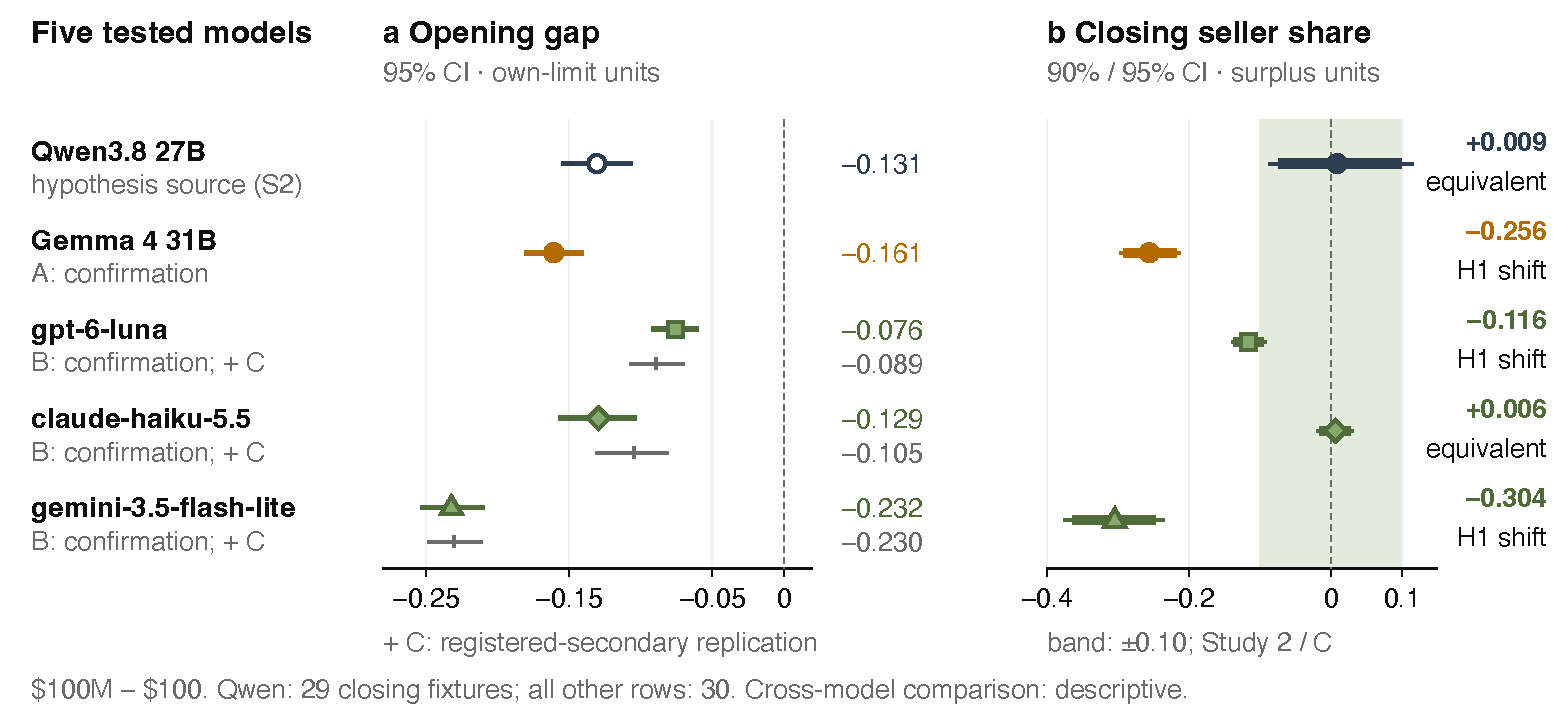
\includegraphics[width=0.92\textwidth]{../manuscript/figures/main_models.pdf}
  \caption{Shared opening modesty, model-dependent closing splits (discovery phase). (a) Mean opening-gap change with 95\% CIs: Qwen is the descriptive hypothesis source; Gemma A and API B estimates are confirmatory; offset API C estimates are registered-secondary replications. (b) Primary closing shifts from Study 2 and C, using all agreements: thick bars 90\%, thin bars 95\%, band $\pm 0.10$.}
  \label{fig:app-models}
\end{figure}

In Addendum C, prospective midpoint accounting (Figure~\ref{fig:app-midpoint}) confirmed tracking (HM2) on all three API models (Spearman $\rho = 0.774, 0.605, 0.847$; Holm $p = 0.00015$ each) and calibration (HM1, $\pm 0.05$) on Luna ($e = -0.009$, 90\% CI [$-0.025, +0.009$]), while Haiku ($+0.025$ [$-0.008, +0.060$]) and Gemini ($-0.043$ [$-0.073, -0.014$]) did not establish $\pm 0.05$ equivalence. Directly clamping openings in Study 3 (Section~\ref{sec:res-clamp}) later tested the causal channel prospectively.

\begin{figure}[t]
  \centering
  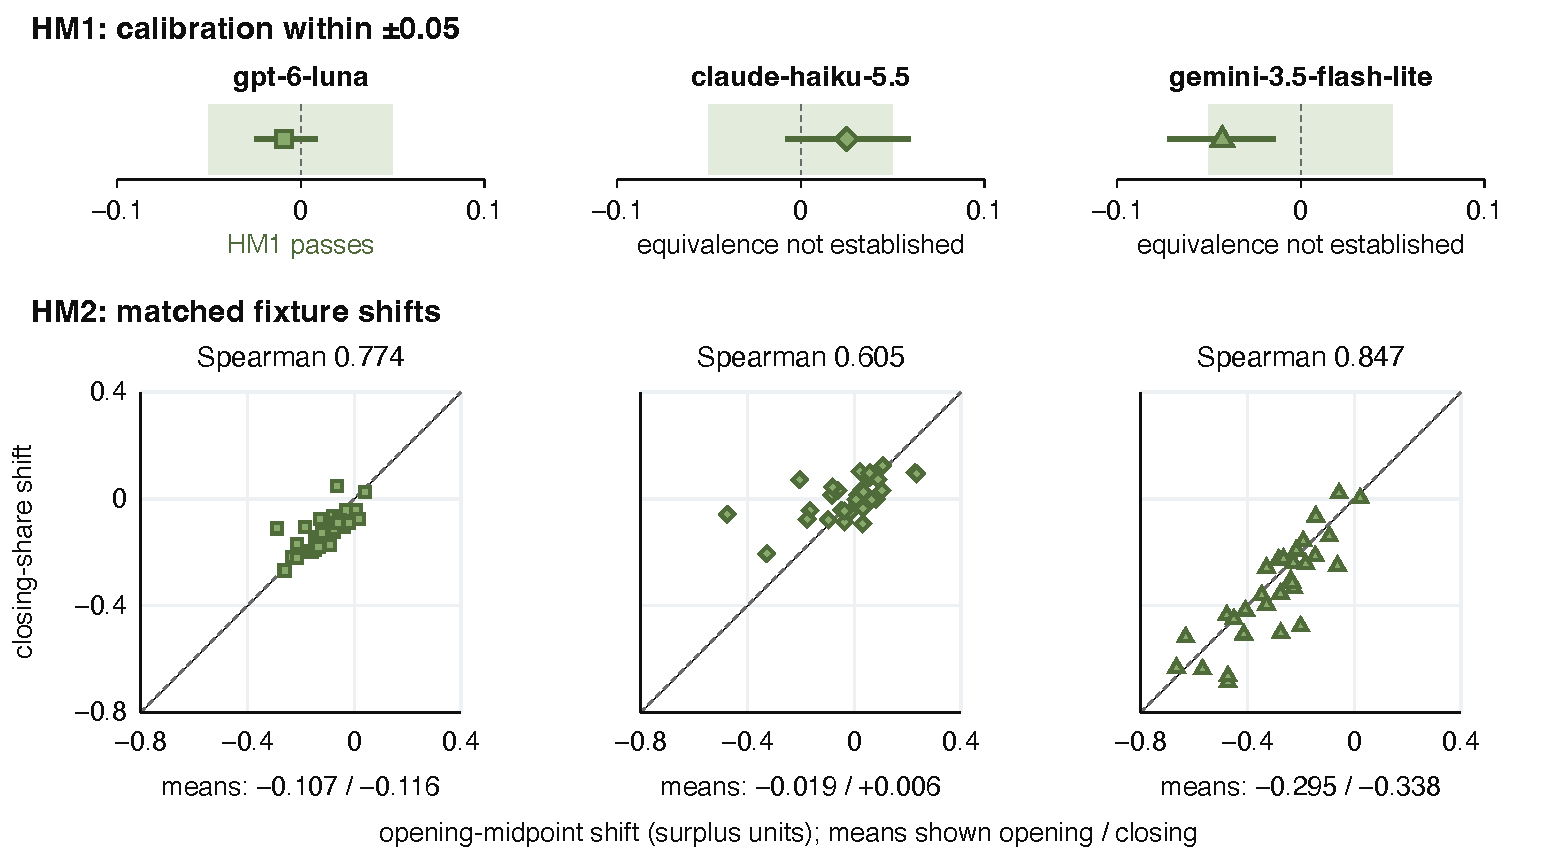
\includegraphics[width=0.90\textwidth]{../manuscript/figures/main_midpoint.pdf}
  \caption{Prospective midpoint accounting in Addendum C. Top: mean closing-minus-midpoint shift with 90\% CI and the $\pm 0.05$ HM1 margin. Bottom: matched fixture shifts (30 per model), with equality shown dashed.}
  \label{fig:app-midpoint}
\end{figure}

\subsection{Exploratory behavioural probes and midpoint decomposition (D.10)}
\label{app:d10}

All analyses in this subsection are exploratory. Figures~\ref{fig:app-probes}, \ref{fig:app-midpoint-open}, \ref{fig:app-map}, and~\ref{fig:app-digits} display the probe results summarised in Section~\ref{sec:res-controls}.

\begin{itemize}
  \item \textbf{Redesigned-game probe (X17, 600 games).} The Study 2 bridge on L01--L30 replicated Gemma's shift ($-0.253$, 95\% CI [$-0.296, -0.209$], 29/30 negative). Redesigned self-play with off-centre ranges, business notation, and cents gave $+0.027$ [$-0.036, +0.088$] after excluding comma-truncated prices (68 slipped games at $\times 10^6$), while both opening gaps still fell (16.5 points for sellers, 9.2 for buyers). Against a scale-invariant scripted bot, Gemma's seller-share change was $-0.258$ [$-0.318, -0.199$] (27/28 fixtures negative).
  \item \textbf{Geometry and notation probes (X18, X22, 2{,}160 games per model).} Crossing Study 2's round-centred zone, a narrow off-centre zone, and a wide zone with raw and business notation gave raw Gemma self-play shifts of $-0.21$, $-0.20$, and $-0.06$ (attenuated by 0.03--0.09 under business notation). Qwen's raw narrow-zone shift was $-0.12$ [$-0.21, -0.03$].
  \item \textbf{Cross-play (X19, 960 games).} Gemma selling to Qwen shifted by $-0.113$, whereas Qwen selling to Gemma shifted by $-0.042$ (non-significant).
  \item \textbf{Instruction probes (X20--X21, 2{,}160 games per model).} Crossing no addition, tough, cooperative, and scale-neutral instructions retained opening shrinkage in every style: 6--13 points for Qwen; 38--47\% of the seller gap and 18--24\% of the buyer gap for Gemma. The exact scale-neutral text was: \emph{``The size of the numbers does not change what good negotiating looks like. Negotiate exactly as you would if every amount were a thousand times smaller or a thousand times larger.''}
  \item \textbf{Information probes (X23--X24, 1{,}560 games per model).} Privately supplying the other side's range pinned Gemma's openings (120/120 buyers at \$75/\$75M; 118/120 sellers at \$120/\$120M) and removed its bot loss (moving from $-0.14$ to $+0.01$; Qwen likewise removed its bot loss). When both sides were told the other's range (X26--X27), Gemma's self-play split still fell by $-0.083 = -0.019 - 0.064$ ($\approx 77\%$ in concessions), whereas Qwen's concession term was $+0.029$ (Figure~\ref{fig:app-midpoint-open}).
  \item \textbf{Digits and cents probes (X15--X16, 1{,}920 + 1{,}680 first moves on Gemma, Y01--Y30).} Keeping digits fixed and changing the unit to millions gave 61\% of the full shift ($-8.9$ of $-14.5$ points; 30/30 negative); changing the digit string at fixed stakes supplied the remaining $-5.6$ points (28/30 negative). Plain small-dollar wording produced 99\% round-ten seller openings (vs.\ 35--57\% under other initial wordings); ``81.00 dollars'' retained 97\% round tens, and adding ``\$'' shifted the both-role gap by only 2--3 points (Figure~\ref{fig:app-digits}).
\end{itemize}

\begin{figure}[t]
  \centering
  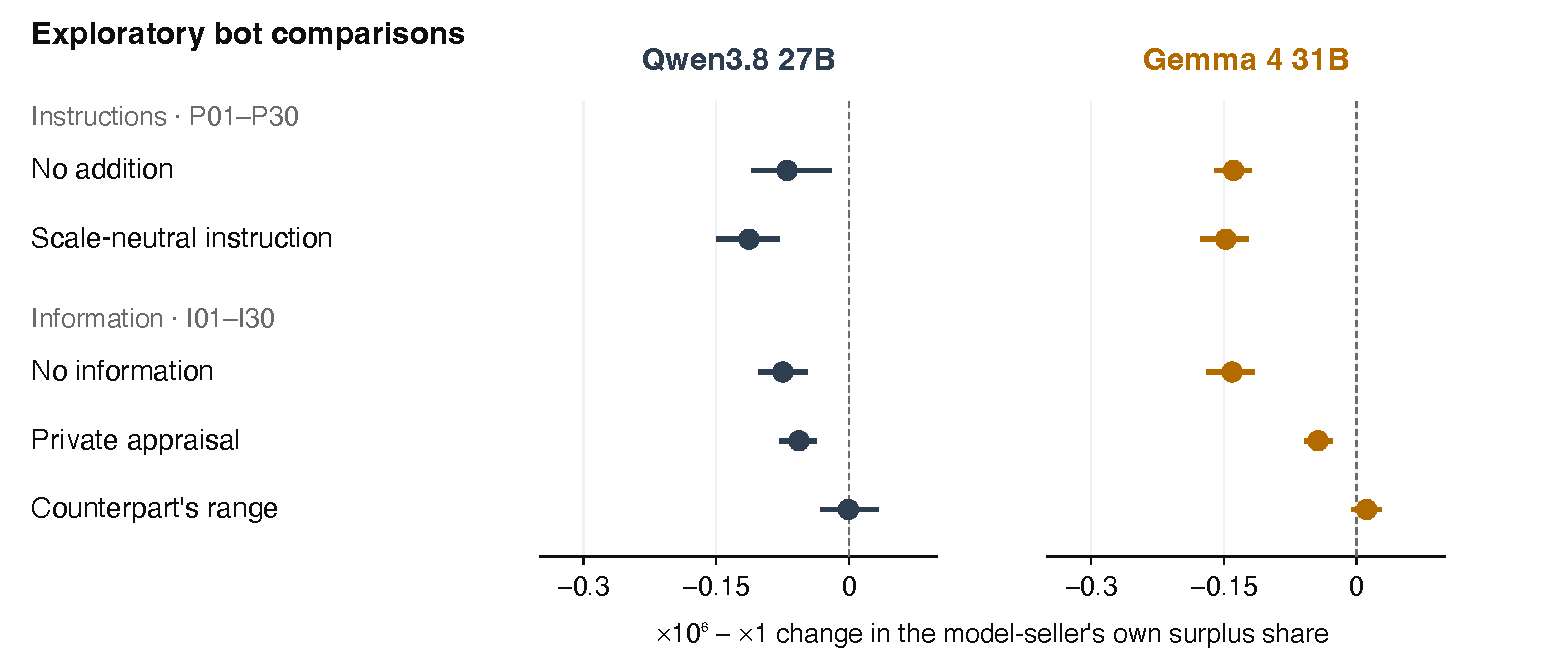
\includegraphics[width=0.90\textwidth]{../manuscript/figures/main_probes.pdf}
  \caption{Instruction and information against a scale-invariant counterpart (exploratory). Change in the model-seller's own surplus share at $\times 10^6$, with 95\% fixture-bootstrap CIs. The scale-neutral instruction retains the loss; knowledge of the counterpart's range removes it in these runs.}
  \label{fig:app-probes}
\end{figure}

\begin{figure}[t]
  \centering
  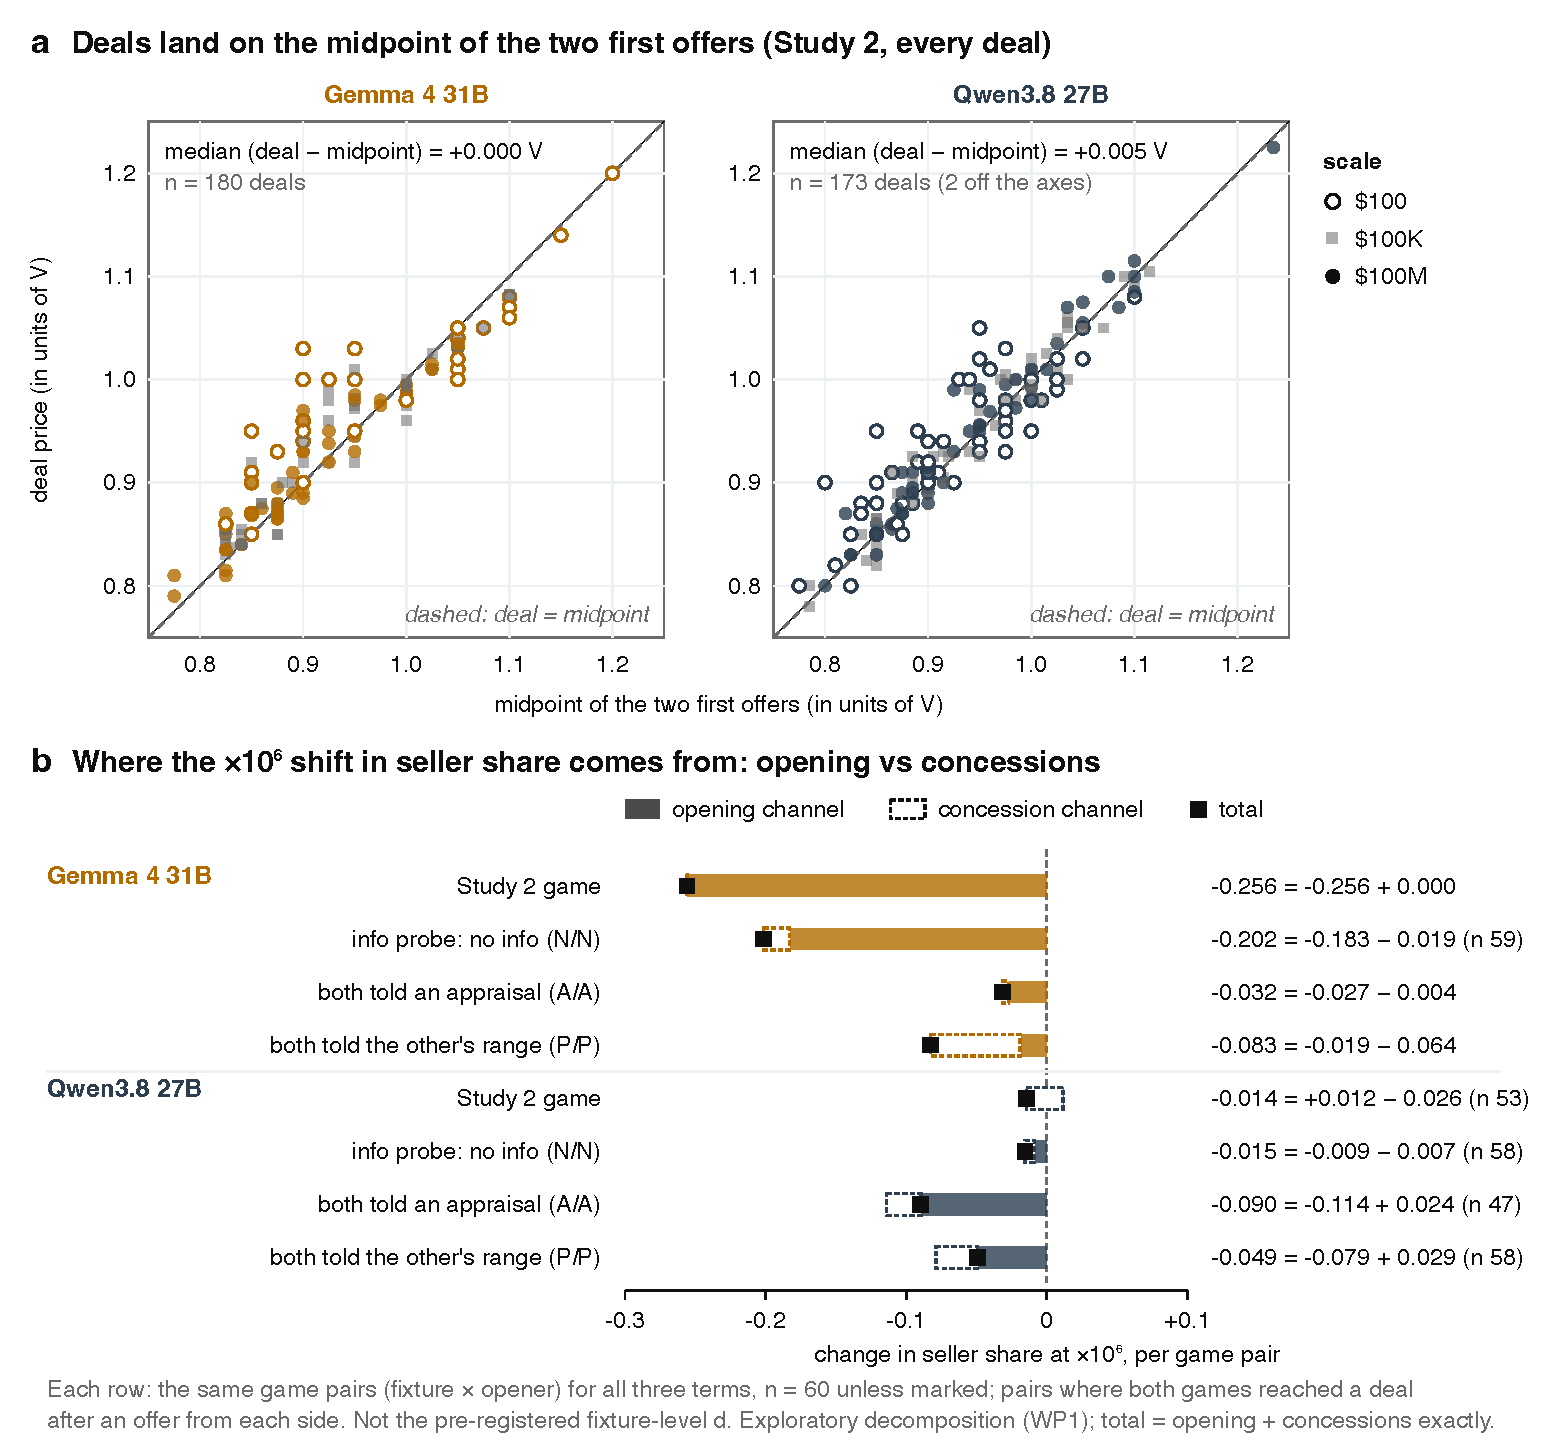
\includegraphics[width=0.90\textwidth]{../manuscript/figures/fig4_midpoint.pdf}
  \caption{Exploratory open-model midpoint and concession accounting. Upper panels compare deals with the in-game first-offer midpoint; lower panel decomposes changes on identical eligible game pairs.}
  \label{fig:app-midpoint-open}
\end{figure}

\begin{figure}[t]
  \centering
  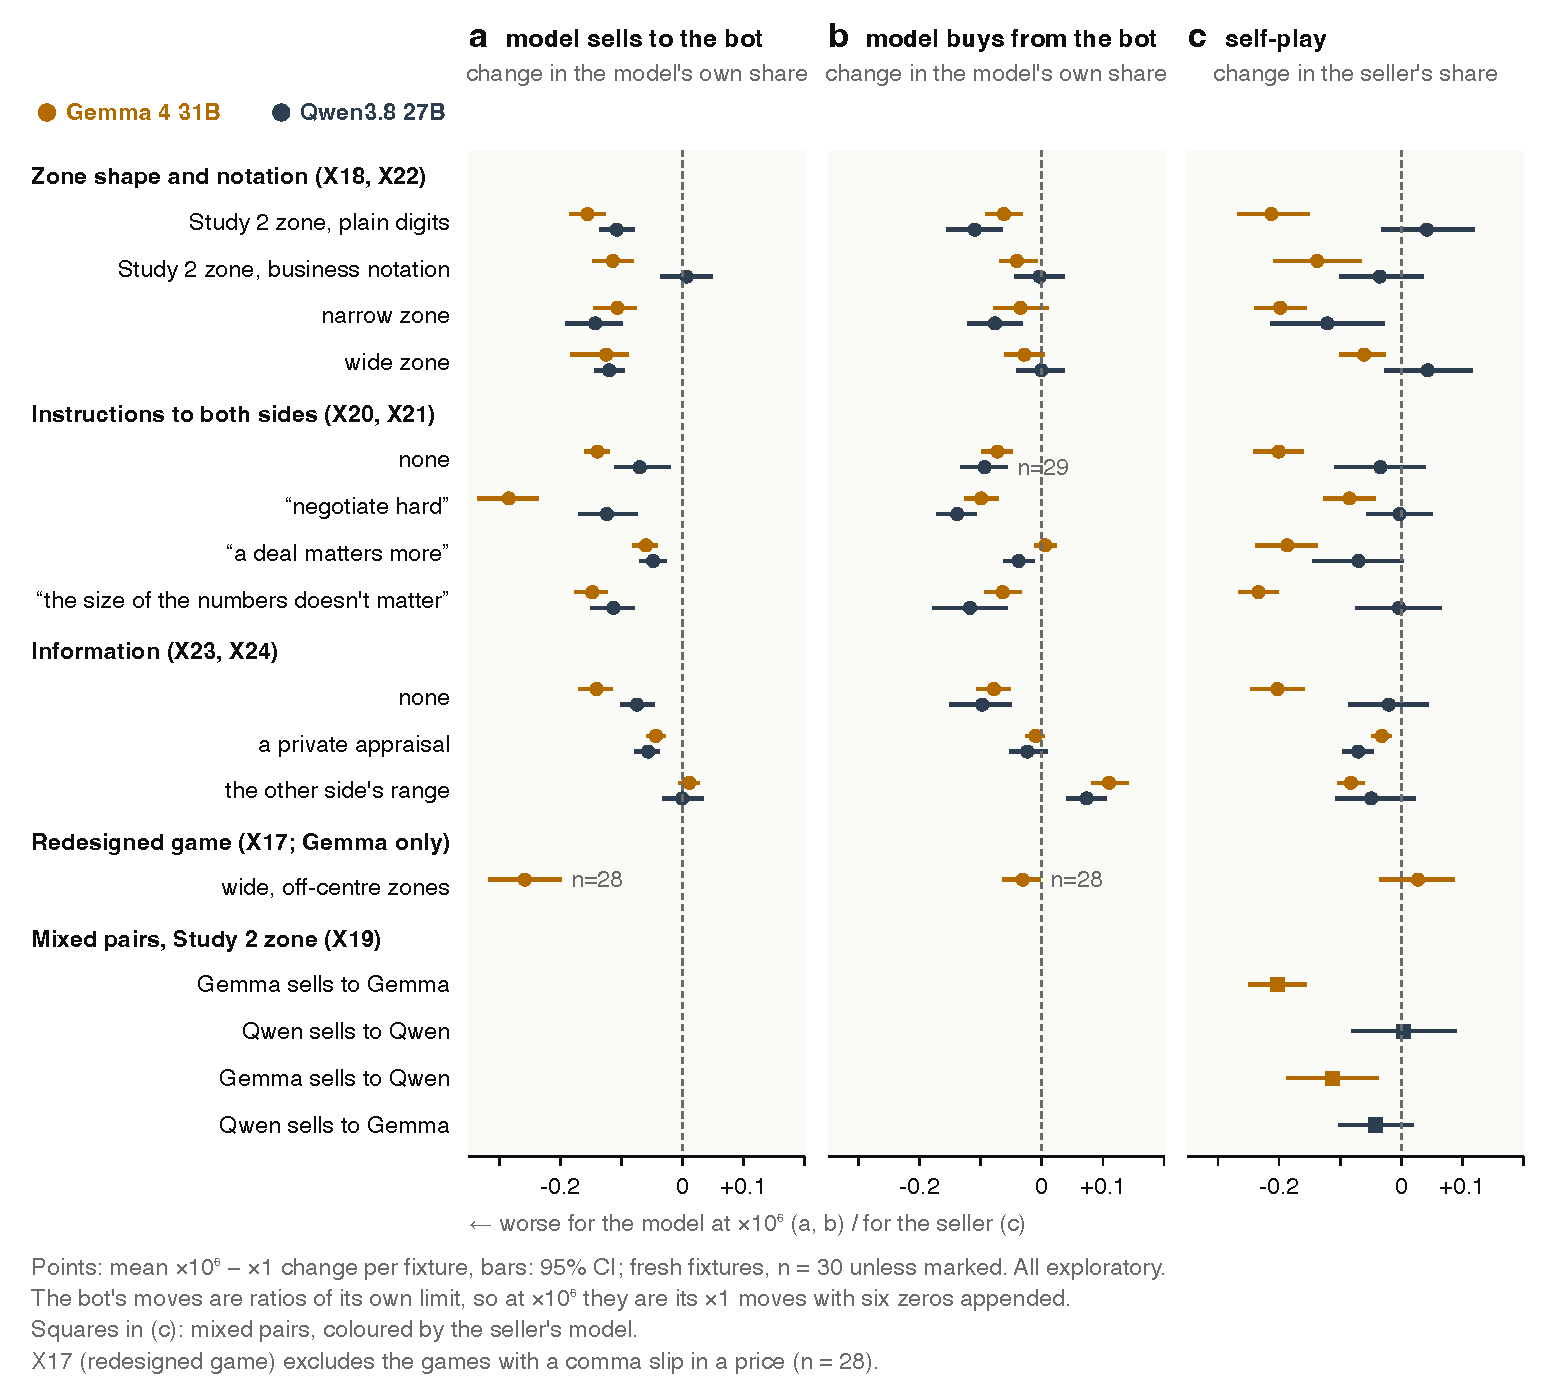
\includegraphics[width=0.92\textwidth]{../manuscript/figures/fig5_map.pdf}
  \caption{Full exploratory behavioural comparison across probe families (95\% CIs). Bot columns use the model's own share, self-play the seller's share.}
  \label{fig:app-map}
\end{figure}

\begin{figure}[t]
  \centering
  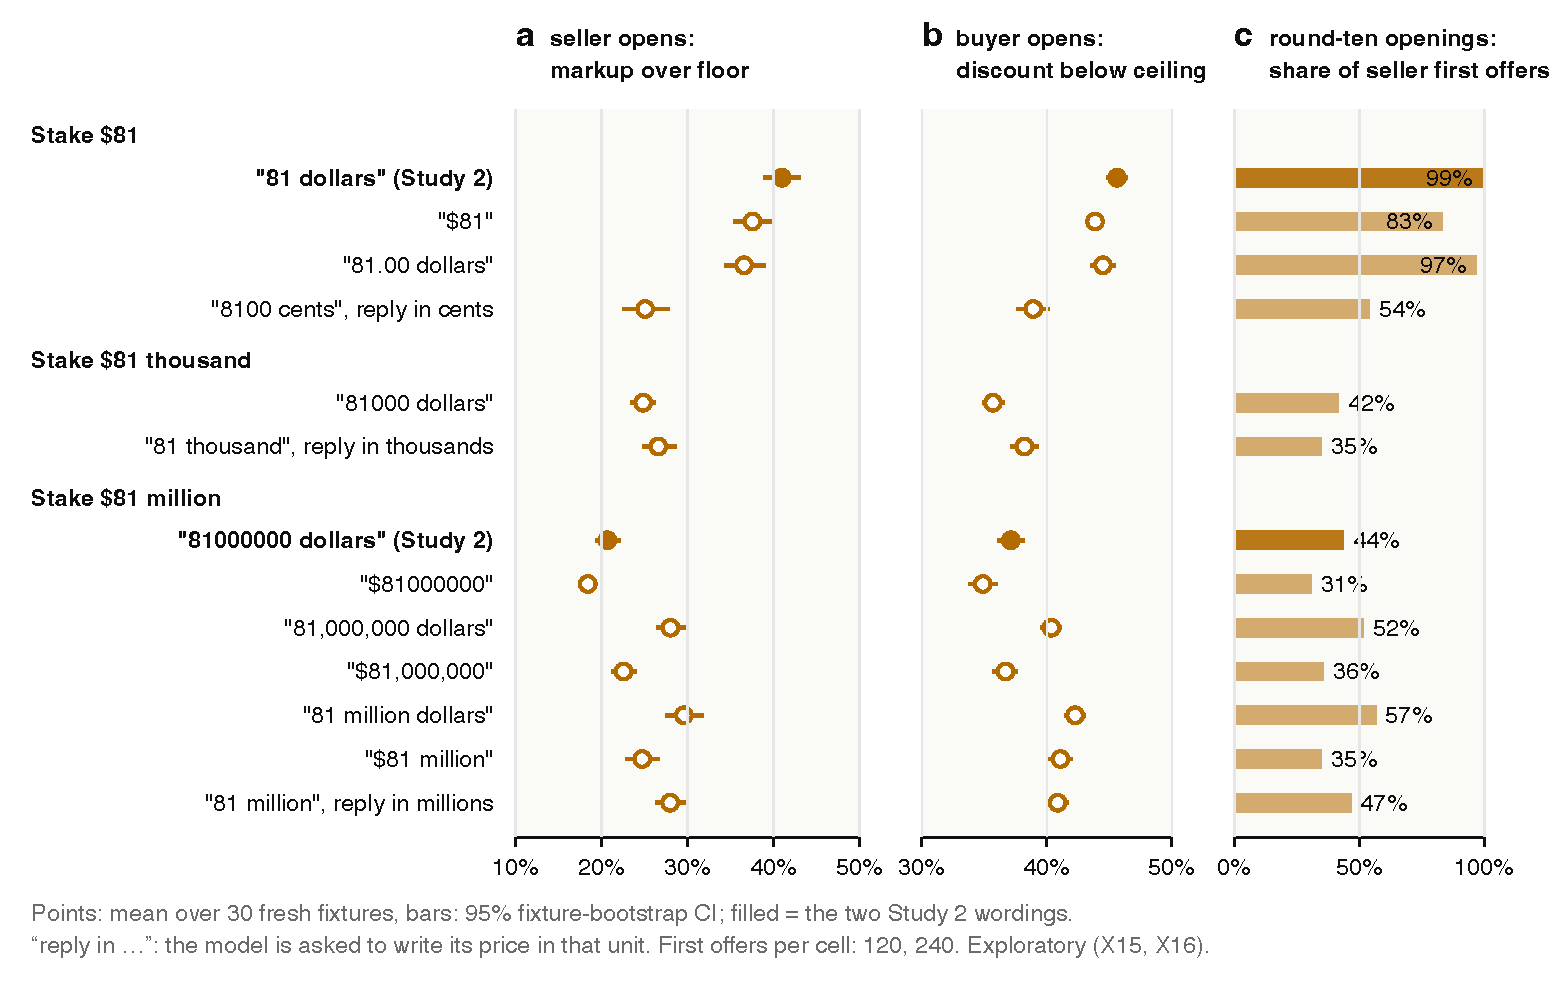
\includegraphics[width=0.92\textwidth]{../manuscript/figures/fig6_digits.pdf}
  \caption{The full 13-wording comparison in Gemma (X15--X16, exploratory). Seller markup, buyer discount, and round-ten seller openings on fresh fixtures (95\% CIs).}
  \label{fig:app-digits}
\end{figure}

\subsection{Discovery-phase mechanistic programme (D.11)}

The discovery-phase mechanistic programme (X51--X64) instrumented Gemma 4 31B in bf16 on 30 fresh fixtures (Y01--Y30). Key findings that motivated E5 and E6: (i) magnitude is linearly decodable from limit digits early ($R^2 = 0.98$--$0.99$ from layer 5; \citealp{belinkov2021probing}), while behavioural patching becomes decisive at layers 41--47 (restoring 82\% [73, 90] of the gap); (ii) prompt-only steering at layer 44 failed ($\le 17\%$), whereas including the reply's 11 opening tokens enabled bidirectional steering of real openings (74--95\% at unit strength across layers 42, 44, and 48; 109--176\% at double strength; non-money control $\le 14\%$; Figure~\ref{fig:app-mech}); (iii) six operationalised concept directions (count, money, million, digits, stakes, modesty) held up to a third of the scale direction's squared norm at layers 41--42, yet their projection moved real openings only 0--6\% while the orthogonal remainder moved 84--86\% (Figure~\ref{fig:app-concepts}; \citealp{singh2024tokenization, elshangiti2024geometry, tan2024steeringreliability, lekeas2026nashcircuit}).

\begin{figure}[t]
  \centering
  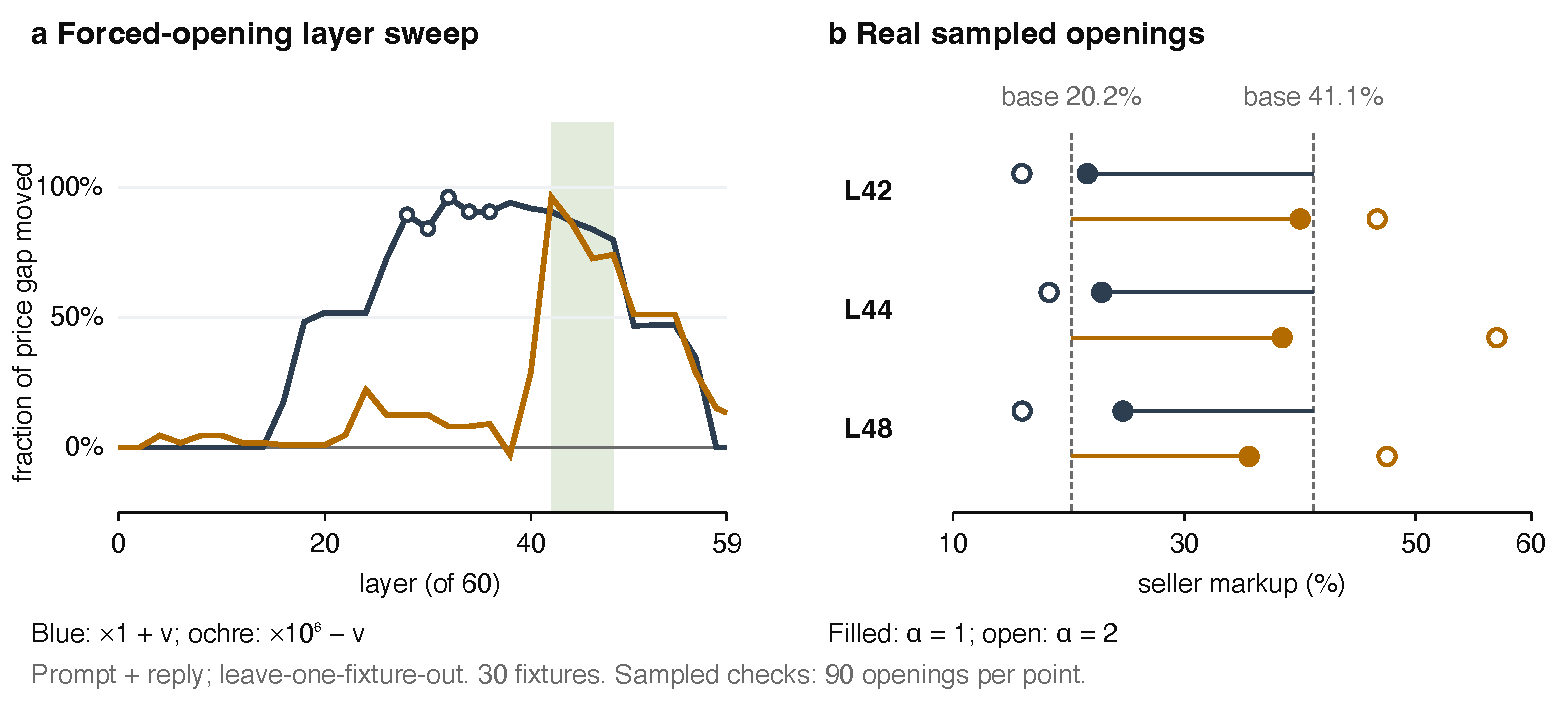
\includegraphics[width=0.92\textwidth]{../manuscript/figures/main_mechanism.pdf}
  \caption{Late bidirectional steering site in Gemma (discovery phase, exploratory). (a) Forced-opening layer sweep; (b) real sampled openings at layers 42, 44, and 48 (all 1{,}080 steered replies format-valid).}
  \label{fig:app-mech}
\end{figure}

\begin{figure}[t]
  \centering
  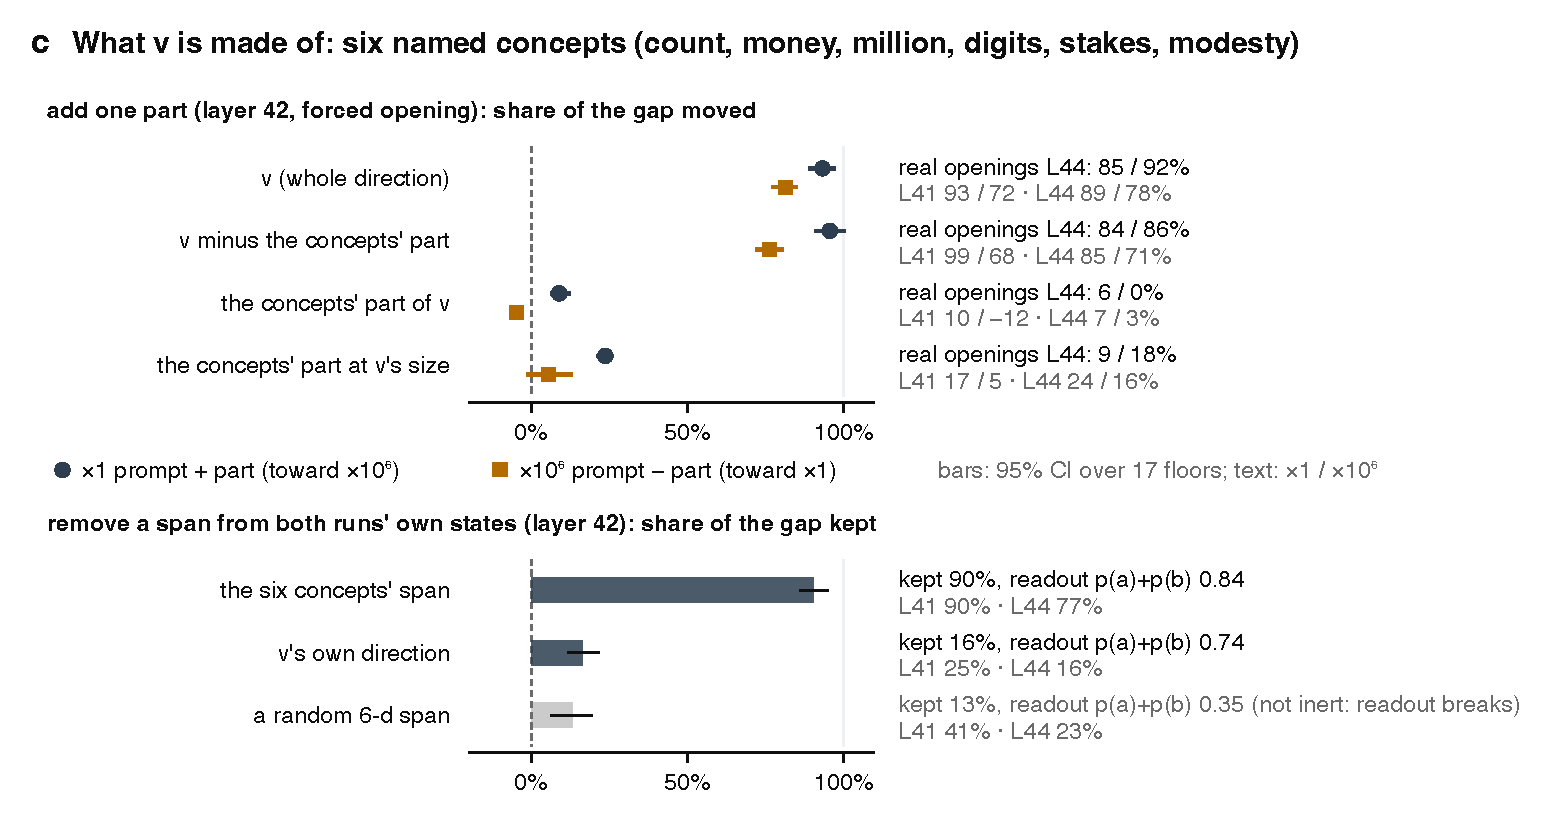
\includegraphics[width=0.92\textwidth]{../manuscript/figures/app_concepts_detail.pdf}
  \caption{Concept projection, orthogonal remainder, and ablation controls on 17 distinct seller floors (X63--X64, exploratory, 95\% CIs).}
  \label{fig:app-concepts}
\end{figure}

\section{E5 methods and full results}
\label{app:e5}

Run \texttt{interp-e5-gemma-4-31b-it-20261015T232511Z} (39 minutes of GPU time, \$1.62 estimated); predictions committed in \texttt{config/interp/e5\_predictions.md} (SHA-256 \texttt{ba05f2c2\ldots}, commit \texttt{0d8b715}) before the run.

\paragraph{Design and readout.} One Study 3 fixture per distinct limit among G01--G40 (19 seller floors: 7 discovery floors G01--G07 and 12 held-out floors; 18 buyer ceilings, 17 usable). Forced openings fix the reply prefix through \texttt{\{"action": "OFFER", "price":} and read the log-odds at the first differing digit between the limit's two A0 greedy prices. Sellers' A0 scale gap is $G_N = 18.4$ nats and A1 gap is $3.0$ nats (17\%; E5-1); buyers' are $7.1$ and $0.7$ nats (10\%). Probability mass on the two deciding tokens is 0.83--0.87 in \$100M runs except buyers' A1 run (\eFiveBuyerProbMass{}).

\begin{table}[t]
  \centering
  \caption{E5 pre-committed exploratory predictions and outcomes.}
  \label{tab:e5-preds}
  \small
  \begin{tabular}{@{}lp{0.50\textwidth}p{0.36\textwidth}@{}}
    \toprule
    ID & Prediction & Outcome \\
    \midrule
    E5-1 & Under A1, sellers' forced opening keeps 5--50\% of the A0 scale gap & Hit: \eFiveGapShare{} \\
    E5-2 & Adding appraisal moves $\le 15\%$ at every layer $\le 39$ and $\ge 50\%$ at L41 or L42 & Hit by signed rule ($+0.5\%$; 83\%); moves 13--35\% wrong way at L30--40 \\
    E5-3 & At L44, reply opening tokens move more than prompt final segment & Hit: \eFiveReplyShare{} vs.\ \eFivePromptShare{} \\
    E5-4 & A0 scale direction moves A1 openings $< 0.5\times$ as much as A0 openings & Hit: \eFiveSteerAoneLow{}--\eFiveSteerAoneHigh{} vs.\ \eFiveSteerAzeroLow{}--\eFiveSteerAzeroHigh{} \\
    E5-5 & $\ge 2$ of top 8 heads shared with scale/range heads; 8 carry $\ge 50\%$ held-out & Overlap hit (\eFiveHeadOverlap{} of 8); reg.\ ratio (\eFiveHeldOutRatio{}) uninterpretable; post-hoc direct share \eFiveHeldOutOwnGapPct{} (12/12 floors) \\
    E5-6 & Buyers show the same onset as E5-2 & Miss: buyers enter gradually from L30 \\
    \bottomrule
  \end{tabular}
\end{table}

% Auto-generated from E5 summary.json
\begin{table}[t]
\centering
\caption{E5 behavioural gate comparing four sampled \texttt{transformers} openings per prompt against Study 3's vLLM openings on the same prompts. Both roles passed the pre-committed gate (all cells and shifts within 3 points; $\ge 95\%$ valid).}
\label{tab:e5-gate}
\footnotesize
\setlength{\tabcolsep}{4pt}
\begin{tabular}{@{}llrrrrrr@{}}
\toprule
Role & Cell & Valid / $n$ & Off-scale & Gap (\texttt{transformers}) & Gap (vLLM) & Prompts & Per-prompt $r$ \\
\midrule
Sellers & A0, \$100 & 76 / 76 & 0 & 44.6\% & 44.5\% & 19 & 0.97 \\
Sellers & A0, \$100M & 76 / 76 & 0 & 22.1\% & 22.5\% & 19 & 0.97 \\
Sellers & A1, \$100 & 76 / 76 & 0 & 37.6\% & 36.7\% & 19 & 1.00 \\
Sellers & A1, \$100M & 76 / 76 & 0 & 34.5\% & 34.1\% & 19 & 0.99 \\
Buyers & A0, \$100 & 72 / 72 & 17 & 44.8\% & 46.0\% & 15 & 0.38 \\
Buyers & A0, \$100M & 72 / 72 & 0 & 35.7\% & 35.9\% & 18 & 0.81 \\
Buyers & A1, \$100 & 72 / 72 & 0 & 31.5\% & 31.6\% & 18 & 0.94 \\
Buyers & A1, \$100M & 72 / 72 & 0 & 24.6\% & 25.1\% & 18 & 0.99 \\
\bottomrule
\end{tabular}
\end{table}

% Auto-generated from E5 summary.json
\begin{table}[t]
\centering
\caption{E5 appraisal swap by layer and token segment at \$100M (share of forced-opening log-odds distance between A0 and A1; sellers 19 floors, buyers 17 ceilings).}
\label{tab:e5-swap}
\small
\begin{tabular}{@{}lrrrr@{}}
\toprule
Layer / segment & Sellers, adding & Sellers, removing & Buyers, adding & Buyers, removing \\
\midrule
0 & $-$2\% & 0\% & 0\% & $-$1\% \\
10 & $-$1\% & $+$1\% & $-$1\% & 0\% \\
20 & $-$1\% & $+$1\% & $-$2\% & $+$1\% \\
24 & $-$3\% & $-$3\% & $-$11\% & $+$4\% \\
26 & $-$8\% & $-$6\% & $-$3\% & $+$7\% \\
28 & $-$13\% & $-$8\% & $+$5\% & $+$7\% \\
30 & $-$13\% & $-$15\% & $+$18\% & $+$13\% \\
32 & $-$20\% & $-$26\% & $+$30\% & $+$19\% \\
34 & $-$26\% & $-$45\% & $+$30\% & $+$25\% \\
36 & $-$30\% & $-$59\% & $+$38\% & $+$42\% \\
37 & $-$36\% & $-$58\% & $+$37\% & $+$43\% \\
38 & $-$35\% & $-$61\% & $+$40\% & $+$49\% \\
39 & $-$27\% & $-$40\% & $+$40\% & $+$65\% \\
40 & $-$23\% & $-$27\% & $+$37\% & $+$63\% \\
41 & $+$75\% & $+$78\% & $+$89\% & $+$79\% \\
42 & $+$83\% & $+$92\% & $+$89\% & $+$82\% \\
43 & $+$87\% & $+$90\% & $+$89\% & $+$82\% \\
44 & $+$88\% & $+$89\% & $+$87\% & $+$82\% \\
46 & $+$89\% & $+$85\% & $+$85\% & $+$82\% \\
48 & $+$99\% & $+$102\% & $+$90\% & $+$84\% \\
52 & $+$104\% & $+$113\% & $+$98\% & $+$95\% \\
56 & $+$105\% & $+$108\% & $+$98\% & $+$98\% \\
59 & $+$111\% & $+$113\% & $+$101\% & $+$103\% \\
\midrule
41, S tokens only & $+$18\% & $+$24\% & $+$21\% & $+$3\% \\
44, S tokens only & $+$22\% & $+$27\% & $+$16\% & $+$3\% \\
48, S tokens only & $+$15\% & $+$23\% & $+$11\% & $+$5\% \\
52, S tokens only & $+$8\% & $+$19\% & $+$11\% & $+$8\% \\
41, reply tokens only & $+$50\% & $+$49\% & $+$77\% & $+$62\% \\
44, reply tokens only & $+$57\% & $+$58\% & $+$78\% & $+$68\% \\
48, reply tokens only & $+$72\% & $+$82\% & $+$80\% & $+$73\% \\
52, reply tokens only & $+$81\% & $+$103\% & $+$88\% & $+$85\% \\
\bottomrule
\end{tabular}
\end{table}

% Auto-generated from E5 summary.json
\begin{table}[t]
\centering
\caption{E5 top eight appraisal-swap heads (layers 38--44, 224 heads) ranked on the 7 discovery floors, and overlap with the discovery-phase scale (X57) and range (X61) head sets (6 of 8 shared; chance $\approx 0.46$).}
\label{tab:e5-heads}
\small
\begin{tabular}{@{}lrcc@{}}
\toprule
Head (layer.head) & Score (discovery) & In scale set (X57) & In range set (X61) \\
\midrule
41.11 & 0.540 & yes & yes \\
41.26 & 0.175 & --- & --- \\
41.8 & 0.130 & --- & yes \\
41.29 & 0.123 & yes & yes \\
43.5 & 0.091 & yes & yes \\
42.9 & 0.077 & yes & --- \\
40.13 & 0.067 & --- & --- \\
39.2 & 0.065 & --- & yes \\
\bottomrule
\end{tabular}
\end{table}

% Auto-generated from E5 held-out circuit table
\begin{table}[t]
\centering
\caption{E5 held-out floors (12): patching the eight appraisal heads' A1 outputs into the A0 \$100M run. Negative moves are toward the \$100 price (12/12 floors). The pre-committed E5-5 ratio ($1.88$) divides by the sign-changing A1 $-$ A0 denominator ($-26.0$ to $+7.1$ nats) and is not a bounded share; the direct share of each floor's own A0 scale gap (mean 67\%, vs.\ 0\% for 8 random heads) is the well-conditioned readout reported in Section~\ref{sec:interp}.}
\label{tab:e5-circuit}
\footnotesize
\setlength{\tabcolsep}{4pt}
\begin{tabular}{@{}lrrrrrr@{}}
\toprule
Floor & Floor (\$100) & 8-head move & Own A0 gap & Share of gap & Reg.\ denom. & 8 rand.\ heads \\
\midrule
G08 & \$93 & $-$5.00 & $+$13.12 & 38\% & $+$5.12 & $+$0.25 \\
G12 & \$78 & $-$17.62 & $+$19.69 & 90\% & $-$22.50 & $-$0.25 \\
G13 & \$80 & $-$13.75 & $+$27.44 & 50\% & $+$0.19 & 0.00 \\
G14 & \$91 & $-$6.12 & $+$12.00 & 51\% & $+$4.25 & 0.00 \\
G15 & \$77 & $-$19.38 & $+$23.06 & 84\% & $-$26.00 & 0.00 \\
G17 & \$86 & $-$15.62 & $+$19.62 & 80\% & $-$11.00 & 0.00 \\
G18 & \$88 & $-$7.50 & $+$13.50 & 56\% & $+$1.25 & $-$0.25 \\
G20 & \$83 & $-$14.00 & $+$16.31 & 86\% & $-$19.25 & $-$0.25 \\
G21 & \$90 & $-$15.75 & $+$22.88 & 69\% & $+$5.38 & $-$0.12 \\
G23 & \$85 & $-$9.38 & $+$13.62 & 69\% & $-$4.00 & $-$0.12 \\
G27 & \$79 & $-$15.88 & $+$18.44 & 86\% & $-$20.75 & 0.00 \\
G37 & \$95 & $-$10.75 & $+$24.62 & 44\% & $+$7.12 & 0.00 \\
\midrule
\textbf{Mean} &  & \textbf{$-$12.56} & \textbf{$+$18.69} & \textbf{67\%} & \textbf{$-$6.68} & \textbf{$-$0.06} \\
\bottomrule
\end{tabular}
\end{table}

\FloatBarrier

\section{E6 methods and full results}
\label{app:e6}

Run \texttt{interp-e6-gemma-4-31b-it-20261016T013146Z} (14 minutes of GPU time, \$0.58 estimated); predictions committed in \texttt{config/interp/e6\_predictions.md} (SHA-256 \texttt{72274e9c\ldots}, commit \texttt{c892fff}) before the run. Table~\ref{tab:e6-preds} scores all ten pre-committed predictions.

\begin{table}[t]
  \centering
  \caption{E6 pre-committed exploratory predictions and outcomes.}
  \label{tab:e6-preds}
  \small
  \begin{tabular}{@{}lp{0.52\textwidth}p{0.34\textwidth}@{}}
    \toprule
    ID & Prediction & Outcome \\
    \midrule
    E6-1 & Negotiation direction (L42, $\alpha = +2$) moves \$100 openings $\ge 40\%$; random $\le 10\%$ & Hit: \eSixNegMove{}; random \eSixNegRand{} \\
    E6-2 & Digits direction reads words and short notation at $r \ge 0.8$ in L10--40 & Hit: $r = 0.97$ (lower of two at best layer) \\
    E6-3 & Transfer to words at L0--2 is $\ge 0.2$ below peak & Hit: $0.61$ vs.\ $0.98$ \\
    E6-4 & Money direction reads people counts at $r \ge 0.8$ & Trivial (L0): $0.94$ already at L0 (shared digits) \\
    E6-5 & Risky choices are safer at \$100M by $\ge 0.5$ nats & Hit: \eSixRiskNatGap{} nats \\
    E6-6 & Direction moves risky choices $\ge 25\%$ of gap and $> 3\times$ controls & Miss: \eSixRiskMove{}; control \eSixRiskCtrl{} \\
    E6-7 & Same for percentage answers & Miss: \eSixPctMove{}; control \eSixPctCtrl{} \\
    E6-8 & Comparisons and sums are intact under the direction & Hit \\
    E6-9 & Fermi estimates move $\le 0.15$ $\log_{10}$ at $\alpha = \pm 2$ & Miss: $+$\eSixFermiPlus{} and $-$\eSixFermiMinus{} (control $+0.97$) \\
    E6-10 & $|\cos(\text{digits direction}, \text{negotiation direction})| \le 0.2$ at L42 & Miss: \eSixCos{} \\
    \bottomrule
  \end{tabular}
\end{table}

\paragraph{Part A (number).} 360 sentences (mantissas 12, 23, 37, 45, 58, 64, 73, 81, 96 $\times$ $10^0$--$10^7$) in five notations (digits, words, short, commas, people count), read at the final period. A magnitude direction is the per-layer covariance of the residual state with $\log_{10}$ amount within one notation; transfer is Pearson $r$ on other notations. The MLP census inspects the down-projection input at layers 4, 10, 20, 30, and 41. Three scoring artefacts: (1) E6-4 transfers at $r = 0.94$ already at layer 0 due to shared digit strings; (2) the pre-committed exponent-tuning count ($z \ge 3$ across 8 exponents) is mathematically unreachable ($\max z = 7/\sqrt{8} \approx 2.47$) and omitted; (3) the random Gaussian vector at $\alpha = \pm 2$ leaves mean probability $0.006$ on valid options in short risk/comparison prompts and breaks parsing on 15/15 percentage prompts in two cells, so its shares there are uninterpretable.

\paragraph{Part B (stakes).} $v_R$ is the mean of the reply-token rows of E5's seller scale difference at layers 42 and 44 ($|v_R| = 30.4$ at layer 42; reply coherence $0.79$); $v_S$ uses the prompt's S tokens ($\cos = 0.85$ with $v_R$); $u$ is the non-money contrast ($\cos = 0.35$); $\text{rand}$ is a seeded Gaussian vector scaled to $|v_R|$. Risky choices by expected-value ratio (safe-option log-odds, mean of 10 prompts): equal EV, $+18.5$ at \$100 and $+20.2$ at \$100M; gamble worth $1.2\times$, $-16.9$ and $-2.6$; gamble worth $1.5\times$, $-11.6$ and $+2.5$. Steered shares at layer 42, $\alpha = +2$, on \$100 prompts: negotiation $v_R$ 86\%, $v_S$ 73\%, $u$ 8\%, rand 8\%; risk $v_R$ 4.9\%, $u$ 1.5\%; percentages $v_R$ $-4.4\%$, $u$ $-2.2\%$. Fermi shifts ($\log_{10}$): $v_R$ $+0.46$ ($\alpha = +1$), $+1.15$ ($+2$), $-0.29$ ($-1$), $-0.50$ ($-2$); $u$ $+0.97$; median item moves $0.04$ at $v_R$ $\alpha = +2$.

% Auto-generated from derived/addendum_d/addendum_d_all.json
\begin{table}[t]
\centering
\caption{E6b layer-covariance-matched, format-orthogonalized random control (\texttt{rand\_cov}, L42, $|\text{rand\_cov}| = |v_R| = 30.39$, $\cos(v_R, \text{rand\_cov}) = 0.000$) vs.\ isotropic \texttt{rand}, non-money control $u$, and negotiation direction $v_R$ at $\alpha = +2$ on \$100 prompts (Gemma 4 31B). Unlike isotropic \texttt{rand} (which collapses valid-option mass to $0.000$), \texttt{rand\_cov} preserves $1.00$ valid-option mass and $100\%$ parse rate while remaining inert on risky choices ($-3.5\%$; $-0.2\%$ at $\alpha=+1$) and percentages ($+2.9\%$).}
\label{tab:e6b}
\footnotesize
\setlength{\tabcolsep}{4.5pt}
\begin{tabular}{@{}llcccc@{}}
\toprule
Family & Metric & $v_R$ (nego) & $u$ (non-money) & \texttt{rand} (isotropic) & \texttt{rand\_cov} (E6b) \\
\midrule
Risk choices & Valid-option mass & 1.00 & 1.00 & 0.00 (broken) & \textbf{1.00} \\
 & Share of natural gap & $+$5\% & $+$2\% & uninterpretable & \textbf{$-$4\%} \\
Comparisons & Valid-option mass & 1.00 & 1.00 & 0.00 (broken) & \textbf{1.00} \\
 & Margin $\Delta$ (nats) & $-$0.74 & $+0.56$ & $-$25.59 & \textbf{$+$0.28} \\
Percentages & Parse valid rate & 100\% & 100\% & breaks at \$100M & \textbf{100\%} \\
 & Share of natural gap & $-$4\% & $-$2\% & $+9\%$ & \textbf{$+$3\%} \\
Sums & Exact-match $\Delta$ & 0.00 & 0.00 & 0.00 & \textbf{0.00} \\
Negotiation & Share of natural gap & $+$86\% & $+$8\% & $+$8\% & \textbf{$+$18\%} \\
\bottomrule
\end{tabular}
\end{table}


\FloatBarrier
\section{Addendum D: Thinking-On, Cross-Play, and \$1{,}000 Anchor Check}
\label{app:addendum-d}

Addendum D (\texttt{prereg/addendum\_d/PREREGISTRATION\_ADDENDUM\_D.md}, frozen in \texttt{prereg/addendum\_d/inputs.sha256} without modifying any of Study 3's 37 hashed files) reuses Study 3's exact 40 fixtures (G01--G40), prompt templates, and reply validator (\texttt{scripts/game\_engine.py}). Block D1 tested native thinking on \texttt{gemini-3.5-flash-lite} (\addDOneGames{} games, \texttt{thinkingBudget=1024}, \texttt{maxOutputTokens=4096}, A0 and A1 at \$100 and \$100M, $k = 2$) plus open-weight pods for Gemma 4 31B and Qwen3.8 27B (\addDOneGemmaGames{} A0 games each within the 45-min pod cap). Block D2 tested all six directed off-diagonal matchups among \{Gemma 4 31B, Qwen3.8 27B, Gemini\} (200 A0 games, 198 agreements, 0 forfeits; Table~\ref{tab:addendum-d2}). Block D3 (\addDThreeGames{} games on Gemini, \texttt{thinkingLevel="MINIMAL"}) tested A0 at \$1{,}000 vs.\ \$100M ($k = 2$). Summary statistics for D1 and D3 are in Table~\ref{tab:addendum-d}, and D2 in Table~\ref{tab:addendum-d2}.

% Auto-generated from derived/addendum_d/addendum_d_all.json
\begin{table}[t]
\centering
\caption{Addendum D2 exploratory 3-model cross-play matrix (200 A0 games across G01--G40, 198 agreements, 0 forfeits; stopped at the 45-min pod cap). Mean seller share at \$100 and \$100M and shift $\Delta = \bar{s}(\$100\text{M}) - \bar{s}(\$100)$ per directed (Seller $\to$ Buyer) pair. High-shrinkage sellers (Gemma, Gemini) lose 16--30 points against Qwen, whereas Qwen selling to Gemini gains $+14$ points.}
\label{tab:addendum-d2}
\footnotesize
\setlength{\tabcolsep}{5pt}
\begin{tabular}{@{}llrrrr@{}}
\toprule
Seller & Buyer & Games & $\bar{s}(\$100)$ & $\bar{s}(\$100\text{M})$ & $\Delta$ (\$100M $-$ \$100) \\
\midrule
Gemini 3.5 FL & Gemma 4 31B & 31 & 0.334 & 0.149 & $-$0.185 \\
Gemini 3.5 FL & Qwen3.8 27B & 46 & 0.384 & 0.225 & $-$0.160 \\
Gemma 4 31B & Gemini 3.5 FL & 41 & 0.489 & 0.381 & $-$0.107 \\
Gemma 4 31B & Qwen3.8 27B & 23 & 0.502 & 0.206 & $-$0.296 \\
Qwen3.8 27B & Gemini 3.5 FL & 32 & 0.313 & 0.452 & $+$0.139 \\
Qwen3.8 27B & Gemma 4 31B & 27 & 0.210 & 0.177 & $-$0.032 \\
\bottomrule
\end{tabular}
\end{table}

\FloatBarrier

\fi

\end{document}
